\documentclass{article}
\usepackage[letterpaper]{geometry}
\usepackage[utf8]{inputenc}
\usepackage[spanish]{babel}
\decimalpoint
\usepackage[dvipsnames]{xcolor}
\usepackage{amsthm}
\usepackage{amssymb}
\usepackage{amsmath}
\usepackage{hyperref}
\usepackage{nicefrac}
\usepackage{bm}
\usepackage[font=small, labelfont=bf, width=.95\textwidth]{caption}
\usepackage{booktabs}
\usepackage{multirow, tabularx}
\usepackage{float}
\usepackage{appendix}
\usepackage{xcolor}
\usepackage{tikz}
\usepackage{tikz-qtree}
\usepackage{setspace}

\hypersetup{
  colorlinks = true,
  linkcolor  = black,
  filecolor  = MidnightBlue,
  citecolor  = MidnightBlue,
  urlcolor   = MidnightBlue
}

\hyphenation{MacOS}

%\usepackage{refcheck}

% Para escribir fácilmente algunos operadores:
\newcommand{\E}{\mathrm{E}}
\newcommand{\var}{\mathrm{var}}
\newcommand{\cov}{\mathrm{cov}}
\newcommand{\der}{\mathrm{d}}

\makeatletter
\newcommand*\bigcdot{\mathpalette\bigcdot@{.5}}
\newcommand*\bigcdot@[2]{\mathbin{\vcenter{\hbox{\scalebox{#2}{$\m@th#1\bullet$}}}}}
\makeatother

\newcolumntype{Y}{>{\centering\arraybackslash}X}

\renewcommand{\appendixpagename}{Apéndices}

\setlength{\parskip}{1em}

\onehalfspacing

\begin{document}

\title{Proyecto final de series de tiempo:\\análisis de la serie \texttt{SP500}}
\author{Rodrigo Leo}
\date{Mayo de 2021}
\maketitle

\begin{abstract}
Este documento presenta un breve análisis estadístico, llevado a cabo en el lenguaje de programación \texttt{R}, de la serie de tiempo del precio y los retornos logarítmicos del índice accionario Standard and Poor's 500, que refleja las condiciones del mercado accionario estadounidense y resulta, por extensión, un buen indicador del estado de los mercados bursátiles mundiales. Se encuentran resultados consistentes con la teoría tradicional de las series de tiempo en lo que respecta a datos financieros de alta volatilidad.
\end{abstract}

\newpage
\tableofcontents

\newpage
\section{Introducción y métodos}

Este documento presenta un análisis de la serie de tiempo del precio del índice accionario Standard and Poor's 500, para el periodo comprendido entre el 4 de enero de 2000 hasta el 20 de abril de 2021, abarcando así un total de 21 años de datos diarios. La serie se obtuvo del sitio web de Yahoo! Finanzas (\url{https://finance.yahoo.com/quote/%5EGSPC}), con periodicidad diaria.

La relevancia de este índice accionario es que representa un excelente indicador de las condiciones del mercado bursátil estadounidense. Esto tiene una conexión directa con mi trabajo de tesis, que estudia el \emph{equity premium puzzle} bajo choques de consumo, y emplea este índice como referencia del retorno de un activo riesgoso representativo. Por este motivo, el análisis de esta serie tiene el potencial de ofrecer una comprensión más profunda de su comportamiento en el largo plazo, y de arrojar luz sobre los resultados de mi proyecto de investigación.

Debido a la imposibilidad de ejecutar una versión suficientemente funcional de \texttt{EViews} en {MacOS}, el trabajo de análisis se llevó a cabo por completo en \texttt{R}. Esto tiene la ventaja de ofrecer un excelente ejercicio de programación en este lenguaje, especializado en análisis estadístico, pero tiene también la desventaja de consumir una cantidad significativamente mayor de tiempo debido a la necesidad de instalar y familiarizarse con paquetes nuevos.

Para que los resultados sean replicables y accesibles, el código en \texttt{R} con el análisis de la serie de tiempo, así como las gráficas y las bases de datos empleadas se encuentran publicados en el siguiente repositorio de \texttt{GitHub}, desde donde se pueden accesar libremente:

\begin{center}
\url{https://github.com/r-leo/proyecto-series}
\end{center}

\newpage
\section{Descripción de la serie de tiempo}

La serie de tiempo se llama \texttt{sp500}, y tiene los parámetros estadísticos mostrados en el cuadro (\ref{tab:parametros_sp500}). Por otra parte, la figura (\ref{fig:sp500}) muestra la gráfica de esta serie.

\begin{figure}[H]
\centering
\includegraphics[width=0.9\textwidth]{../figuras/sp500.png}
\caption{\label{fig:sp500}Gráfica de la serie de tiempo \texttt{sp500}.}
\end{figure}

Se puede observar fácilmente que la serie presenta una tendencia ascendente clara. Existen caídas importantes en el año 2000 (debida a la crisis \emph{dotcom}) y en el año 2009 (debida a la crisis financiera originada en Estados Unidos). Se observa también una caída fuerte alrededor del año 2019 seguida de una rápida recuperación. Esta última caída se asocia a la crisis provocada por la pandemia del COVID-19.

\begin{table}[H]
\centering
\begin{tabularx}{0.5\textwidth}{XY}
\toprule
Parámetro & Valor \\
\midrule
Mínimo & 676.5 \\
Máximo & 4185.5 \\
Media & 1684.8 \\
\bottomrule
\end{tabularx}
\caption{\label{tab:parametros_sp500}Parámetros estadísticos de la serie \texttt{sp500}.}
\end{table}

Aunque el gráfico muestra una tendencia clara, para probar formalmente la estacionariedad de la serie se emplea la prueba aumentada de Dickey-Fuller. Como resultado se obtiene un valor del estadístico de -0.49676 para un regazo de 17 periodos, que se traduce en un valor $p$ de 0.982. El valor $p$ cercano a uno indica que no se puede rechazar la hipótesis nula de que la serie presenta una raíz unitaria.

Para tratar de corregir este efecto, se obtiene la serie de las primeras diferencias logarímicas, que corresponen a los retornos logarítmicos del activo. Esta serie se denota \texttt{sp500-1}. La figura (\ref{fig:sp500_1}) muestra la gráfica de esta nueva serie.

\begin{figure}[H]
\centering
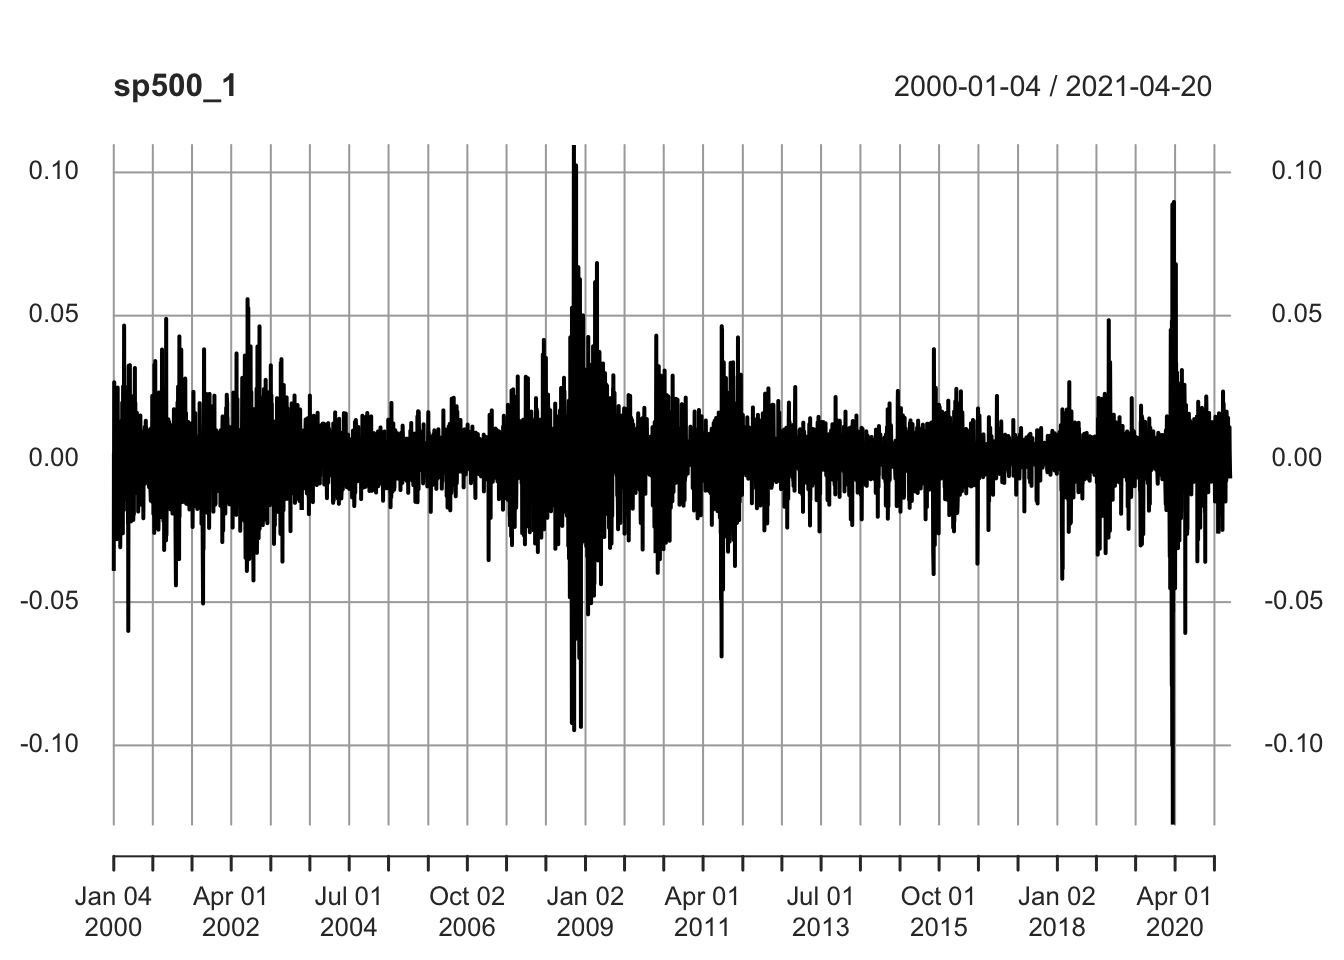
\includegraphics[width=0.9\textwidth]{../figuras-log/sp500_1.png}
\caption{\label{fig:sp500_1}Gráfica de la serie de tiempo \texttt{sp500-1}, que corresponde a las primeras diferencias logarítmicas de la serie \texttt{sp500}.}
\end{figure}

Al realizar la prueba aumentada de Dickey-Fuller sobre esta nueva serie se obtiene un valor del estadístico de -17.641, para un rezago de 17 periodos, que corresponde a un valor $p$ de 0.01. Por lo tanto, la serie de primeras diferencias logarítmicas \texttt{sp500-1} no tiene raíz unitaria, con un nivel de significancia $\alpha = 0.05$.

Al obtener las funciones de autocorrelación y autocorrelación parcial de la serie \texttt{sp500-1}, se observa que la serie presenta autocorrelación significativa. Las figuras (\ref{fig:sp500_1_acf}) y (\ref{fig:sp500_1_pacf}) muestran estas funciones de autocorrelación y autocorrelación parcial, respectivamente.

\begin{figure}[H]
\centering
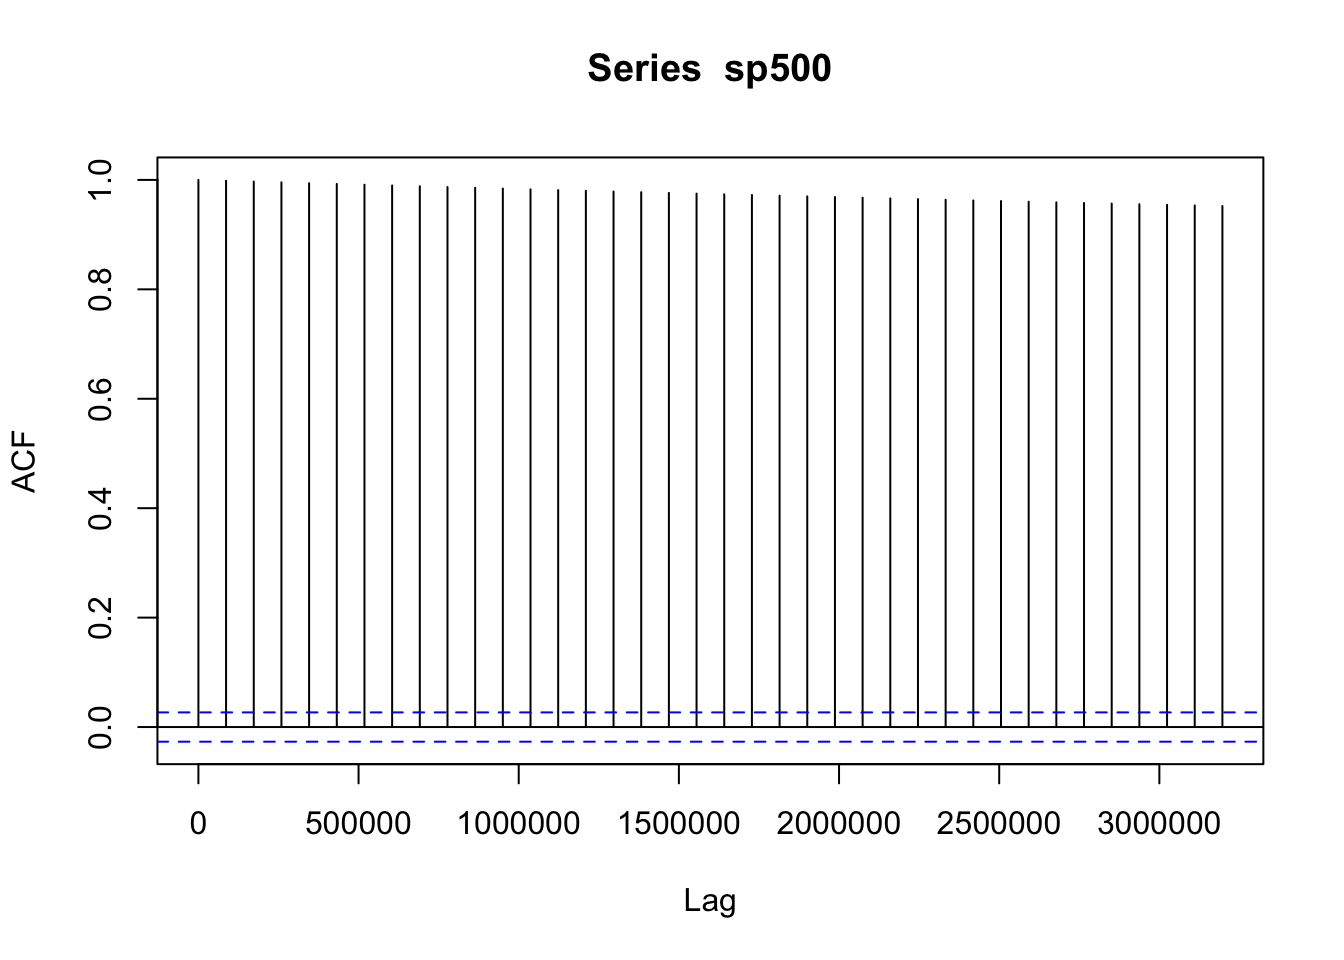
\includegraphics[width=0.9\textwidth]{../figuras-log/sp500_1_acf.png}
\caption{\label{fig:sp500_1_acf}Gráfica de la función de autocorrelación de la serie \texttt{sp500-1}.}
\end{figure}

\begin{figure}[H]
\centering
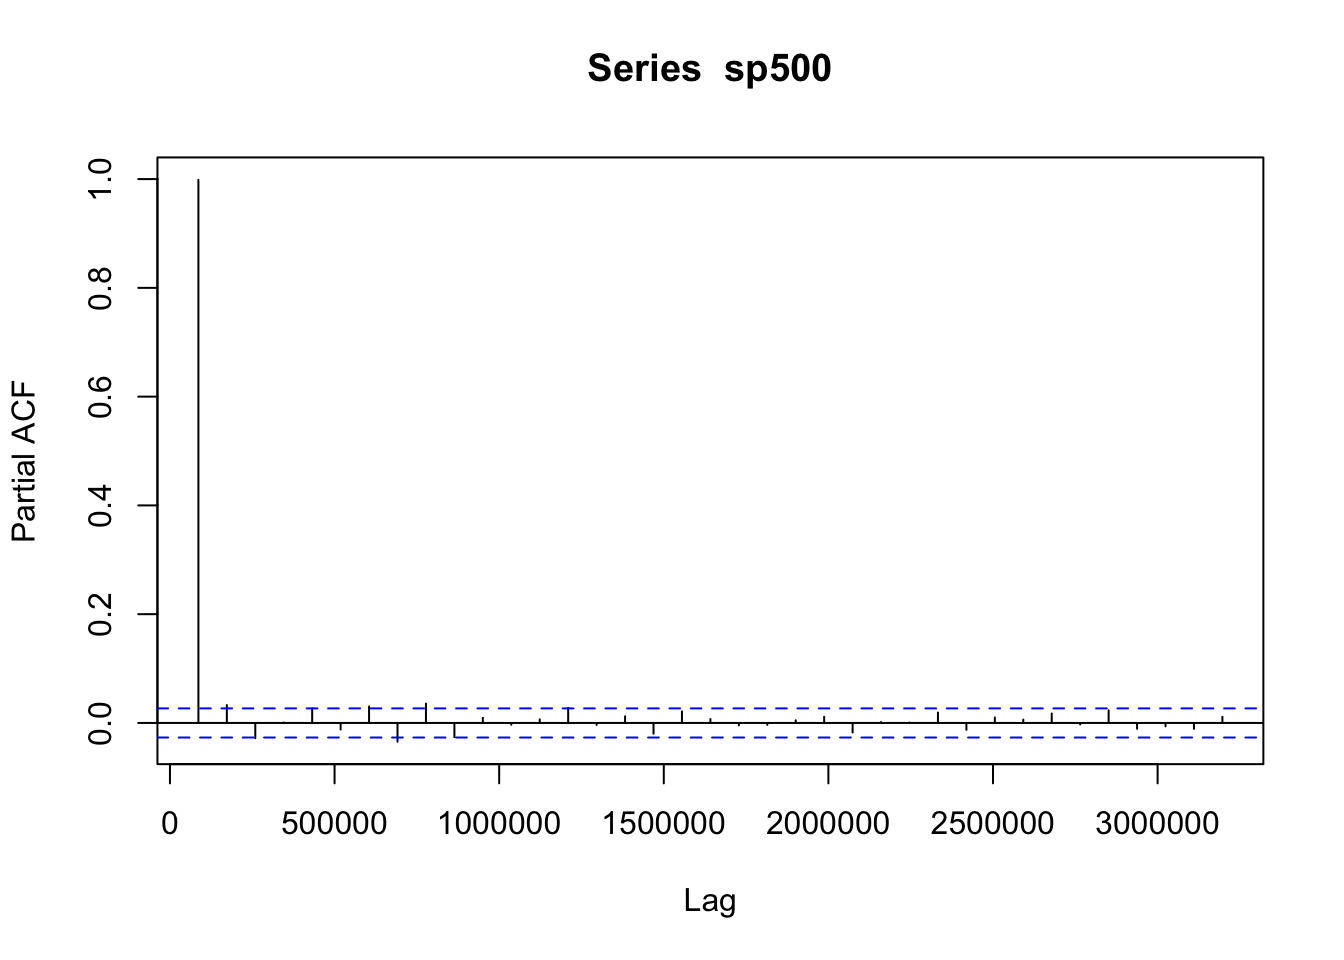
\includegraphics[width=0.9\textwidth]{../figuras-log/sp500_1_pacf.png}
\caption{\label{fig:sp500_1_pacf}Gráfica de la función de autocorrelación parcial de la serie \texttt{sp500-1}.}
\end{figure}

Con el propósito de probar formalmente la existencia de autocorrelación serial, se lleva a cabo la prueba de Ljung-Box para órdenes de rezago desde 1 hasta 10. Los resultados se muestran en la tabla (\ref{tab:ljungbox}).

\begin{table}[H]
\centering
\begin{tabularx}{0.9\textwidth}{YYY}
\toprule
Orden & Estadístico de Ljung-Box & Valor $p$ \\
\midrule
1 & 68.8 & 1.110223e-16 \\
2 & 68.9 & 1.110223e-15 \\
3 & 70.1 & 3.996803e-15 \\
4 & 73.3 & 4.551914e-15 \\
5 & 74.3 & 1.276756e-14 \\
6 & 81.9 & 1.44329e-15 \\
7 & 87.8 & 3.330669e-16 \\
8 & 92.5 & 1.110223e-16 \\
9 & 100.3 & 0 \\
10 & 100.3 & 0 \\
\bottomrule
\end{tabularx}
\caption{\label{tab:ljungbox}Resultados de la prueba de Ljung-Box sobre la serie \texttt{sp500-1}, para probar la existencia de autocorrelación.}
\end{table}

La prueba de Ljung-Box se realizó hasta el orden 30, obteniendo en todos los casos un valor $p$ menor a 0.05. Esto indica que se rechaza la hipótesis nula de que las observaciones de la serie no tienen autocorrelación serial para órdenes menores o iguales a 30. Esto confirma lo observado en las gráficas de las figuras (\ref{fig:sp500_1_acf}) y (\ref{fig:sp500_1_pacf}).

La existencia de autocorrelación sugiere que el uso de un modelo autorregresivo $\mathrm{AR}(p)$ puede dar buenos resultados para modelar esta serie de tiempo.


\newpage
\section{Modelo ARMA}

La especificación más general de un modelo $\mathrm{ARMA}(p, q)$ es
\[ y_t = a_0 + a_1 y_{t-1} + \cdots + a_p y_{t-p} + b_1 e_{t-1} + \cdots + b_q e_{t-q} + e_t \]
donde $e_{t} \sim N \ \forall t$.

Dado que en \texttt{R} sólo se pueden calcular criterios de información para modelos $\mathrm{ARIMA}(p, d, q)$ estimados mediante máxima verosimilitud (MLE), este será el método de estimación que se empleará para ajustar la serie al modelo. Sin embargo, dado que trabajamos con una serie estacionaria, el orden de diferencia del modelo $\mathrm{ARIMA}(p, d, q)$ será cero, lo que equivale a un modelo $\mathrm{ARMA}(p, q)$.

En primer lugar se estima el modelo $\mathrm{ARMA}(1, 1)$, obteniendo los siguientes coeficientes:

\begin{table}[H]
\centering
\begin{tabularx}{0.7\textwidth}{YYY}
\toprule
\texttt{ar1} & \texttt{ma1} & \texttt{media} \\
\midrule
0.0071 & -0.1225 & 2e-04 \\
(0.1140) & (0.1132) & (2e-04) \\
\bottomrule
\end{tabularx}
\caption{\label{tab:arma-1-1}Coeficientes de la estimación del modelo ARMA(1, 1). Los valores entre paréntesis son errores estándar.}
\end{table}

A este modelo le corresponde una $\sigma^2$ estimada de 0.0001546, un valor de log-likelihood de 15,902.42, y los siguientes valores de criterios de información:
\begin{itemize}
\item Criterio de información de Akaike (AIC): -31,796.83.
\item Criterio de información bayesiano (BIC): -31,770.49.
\end{itemize}

Para determinar la mejor combinación de parámetros $(p, q)$, se estimaron 100 modelos $\mathrm{ARMA}(p, q)$, variando ambos parámetros de forma independiente entre 1 y 10 y calculando el valor del criterio de información de Akaike para cada modelo. Los resultados fueron los siguientes:

\begin{table}[H]
\centering
\begin{tabularx}{0.9\textwidth}{YYYYYY}
\toprule
\multirow{2}{*}{$p$} & \multicolumn{5}{c}{$q$} \\
\cmidrule{2-6}
& 1 & 2 & 3 & 4 & 5 \\
%\midrule
1 & -31796.83 & -31794.85 & -31797.92 & -31799.09 & -31797.62 \\
2 & -31794.97 & -31793.88 & -31792.37 & -31798.09 & -31797.17 \\
3 & -31793.83 & -31791.83 & -31793.82 & -31801.75 & -31799.75 \\
4 & -31798.27 & -31800.00 & -31801.23 & -31799.93 & -31804.20 \\
5 & -31797.20 & -31797.85 & -31799.79 & -31805.14 & -31824.08 \\
6 & -31808.80 & -31814.52 & -31815.80 & -31816.47 & -31813.69 \\
7 & -31807.15 & -31804.92 & -31811.22 & -31815.32 & -31815.08 \\
8 & -31806.75 & -31820.05 & -31801.15 & -31826.01 & -31824.20 \\
9 & -31808.56 & -31830.77 & -31825.19 & -31820.85 & -31824.14 \\
10 & -31806.61 & -31804.60 & -31830.82 & -31828.03 & -31817.85 \\
\midrule
\multirow{2}{*}{$p$} & \multicolumn{5}{c}{$q$} \\
\cmidrule{2-6}
& 6 & 7 & 8 & 9 & 10 \\
1 & -31805.47 & -31804.77 & -31803.20 & -31804.44 & -31802.50 \\
2 & -31815.28 & -31802.85 & -31818.27 & -31802.54 & -31800.50 \\
3 & -31815.01 & -31811.51 & -31815.39 & -31817.91 & -31817.64 \\
4 & -31815.45 & -31815.01 & -31809.93 & -31810.88 & -31823.46 \\
5 & -31822.41 & -31819.64 & -31821.80 & -31830.96 & -31841.80 \\
6 & -31821.95 & -31829.05 & -31820.85 & -31827.64 &-31836.98 \\
7 & -31829.58 & -31826.89 & -31835.50 & -31830.42 & -31834.89 \\
8 & -31822.00 & -31823.08 & -31831.50 & -31831.22 & -31834.37 \\
9 & -31833.60 & -31832.09 & -31831.05 & -31844.89 & -31840.76 \\
10 & -31828.08 & -31829.97 & -31836.79 & -31843.16 & -31841.25 \\
%\midrule
\bottomrule
\end{tabularx}
\caption{\label{tab:akaike}Valores del criterio de información de Akaike (AIC) para el modelo $\mathrm{ARMA}(p, q)$, donde el valor de $p$ es el número de fila y el valor de $q$ es el número de columna.}
\end{table}

A partir de los resultados del cuadro (\ref{tab:akaike}), se observa que el valor mínimo del criterio de información es -31,844.89, que corresponde a la entrada $p=9$, $q=9$. Por lo tanto, se considera que el mejor modelo para esta serie es $\mathrm{ARMA}(9, 9)$.

Al estimar el modelo $\mathrm{ARMA}(9, 9)$ seleccionado se obtienen los siguientes coeficientes:

\begin{table}[H]
\centering
\begin{tabularx}{0.6\textwidth}{XYY}
\toprule
Coeficiente & Valor & Error estándar \\
\midrule
\texttt{ar1} & 0.1031 & 0.0706 \\
\texttt{ar2} & -0.3081 & 0.0387 \\
\texttt{ar3} & 0.5003 & 0.0796 \\
\texttt{ar4} & 0.3950 & 0.0872 \\
\texttt{ar5} & -0.2157 & 0.0602 \\
\texttt{ar6} & -0.5844 & 0.0674 \\
\texttt{ar7} & 0.1778 & 0.0805 \\
\texttt{ar8} & -0.4054 & 0.0611 \\
\texttt{ar9} & 0.3980 & 0.0694 \\
\texttt{ma1} & -0.2165 & 0.0690 \\
\texttt{ma2} & 0.3167 & 0.0623 \\
\texttt{ma3} & -0.5186 & 0.0937 \\
\texttt{ma4} & -0.3737 & 0.1013 \\
\texttt{ma5} & -0.2616 & 0.0786 \\
\texttt{ma6} & 0.5165 & 0.0806 \\
\texttt{ma7} & 0.1524 & 0.0754 \\
\texttt{ma8} & 0.3641 & 0.0649 \\
\texttt{ma9} & -0.3697 & 0.0747 \\
\texttt{Media} & 2e-04 & 1e-04 \\
\bottomrule
\end{tabularx}
\caption{\label{tab:arma-9-9}Coeficientes de la estimación del modelo ARMA(9, 9). Los valores entre paréntesis son errores estándar.}
\end{table}

A este modelo le corresponde una $\sigma^2$ estimada de 0.0001528, un valor de log-likelihood de 15m942.44, y los siguientes valores de criterios de información:
\begin{itemize}
\item Criterio de información de Akaike (AIC): -31,844.89.
\item Criterio de información bayesiano (BIC): -31,713.17.
\end{itemize}

Para evaluar si el modelo $\mathrm{ARMA}(9, 9)$ seleccionado es adecuado, se verifica que los residuales sean ruido blanco. La figura (\ref{fig:residuales}) muestra la gráfica de los mismos, así como su función de autocorrelación y su histograma. Se observa que parece existir autocorrelación, lo cual indicaría que los residuales no son ruido blanco y por lo  tanto el modelo seleccionado no es capaz de capturar adecuadamente la información de la serie.

Para verificar formalmente la posible autocorrelación de los residuales, se lleva a cabo la prueba de Ljung-Box, la cual resulta en un estadístico $Q^* = 21.2$ para 22 rezagos, que equivale  a un valor $p$ de $9.567 \times 10^{05} \approx 0$. Por lo tanto no se puede rechazar la hipótesis nula de que los residuales del modelo ajustado presentan autocorrelación, y por lo tanto no puede asumirse que sean ruido blanco, lo cual invalida el modelo seleccionado.

\begin{figure}[H]
\centering
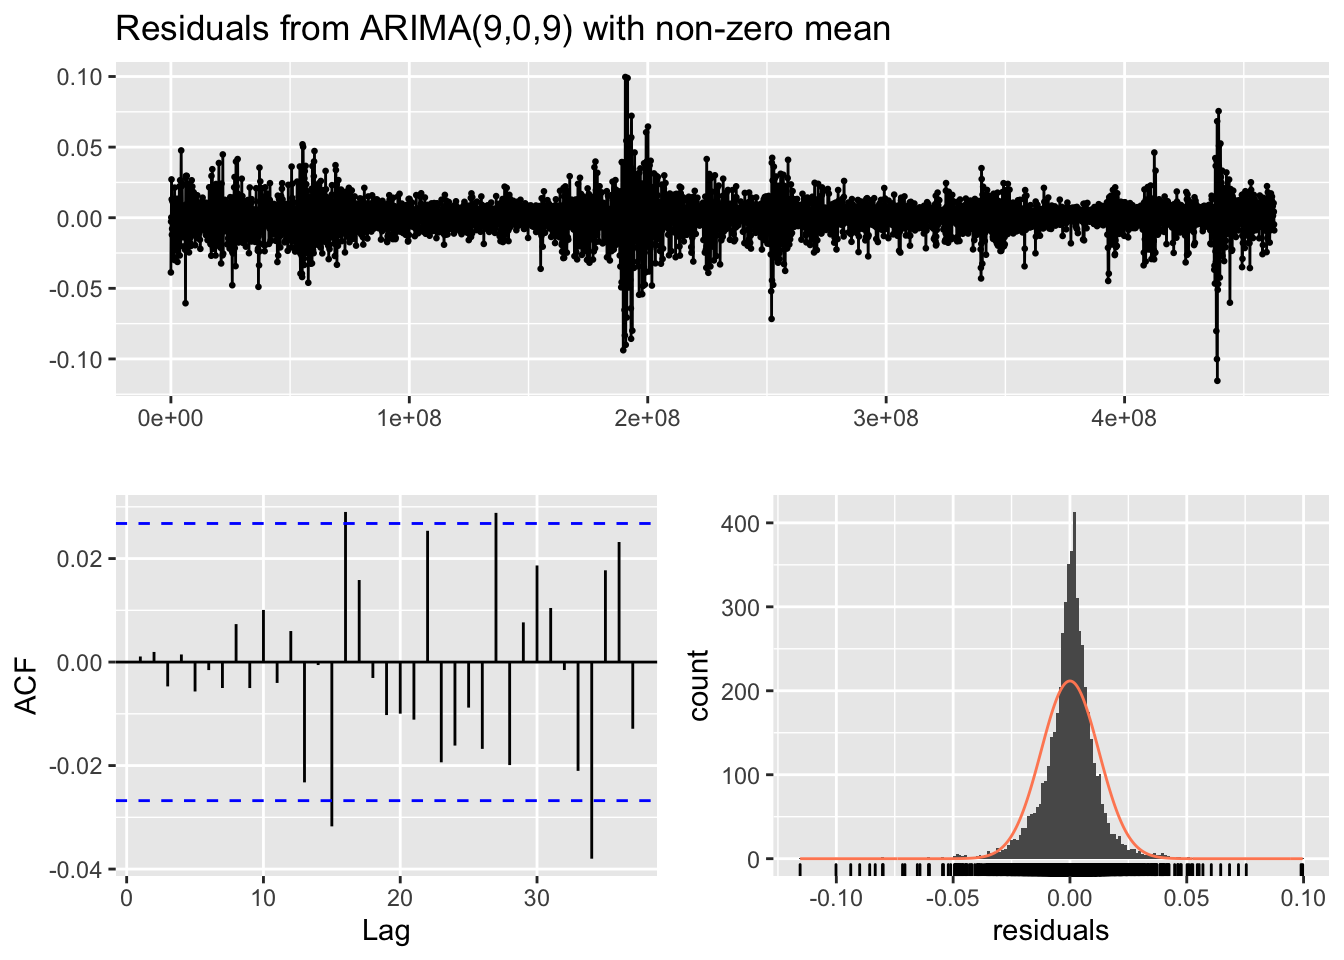
\includegraphics[width=0.9\textwidth]{../figuras-log/residuales.png}
\caption{\label{fig:residuales}Gráfica de los residuales del modelo $\mathrm{ARMA(4, 4)}$, su autocorrelación y su histograma, para la serie \texttt{sp500-1}.}
\end{figure}

Para tratar de solucionar el problema que presenta el modelo se puede optar por tratar de encontrar un mejor ajuste empleando órdenes $(p, q)$ mayores. Sin embargo, dado que la serie es de frecuencia diaria y se trata de un índice del mercado financiero que opera un gran volumen diario, es posible que las dificultades del ajuste provengan de la fuerte volatilidad diaria de la serie. Por lo tanto, se propone reducir la frecuencia de los datos a periodicidad mensual empleando el valor de cierre del último día del mes como la observación mensual correspondiente. Esta nueva serie se denomina \texttt{sp500m}.

La figura (\ref{fig:sp500m}) muestra la gráfica de esta serie de tiempo. Es fácil observar que la volatilidad es menor si se compara visualmente con la figura (\ref{fig:sp500}), que corresponde a la serie original de frecuencia diaria.

\begin{figure}[H]
\centering
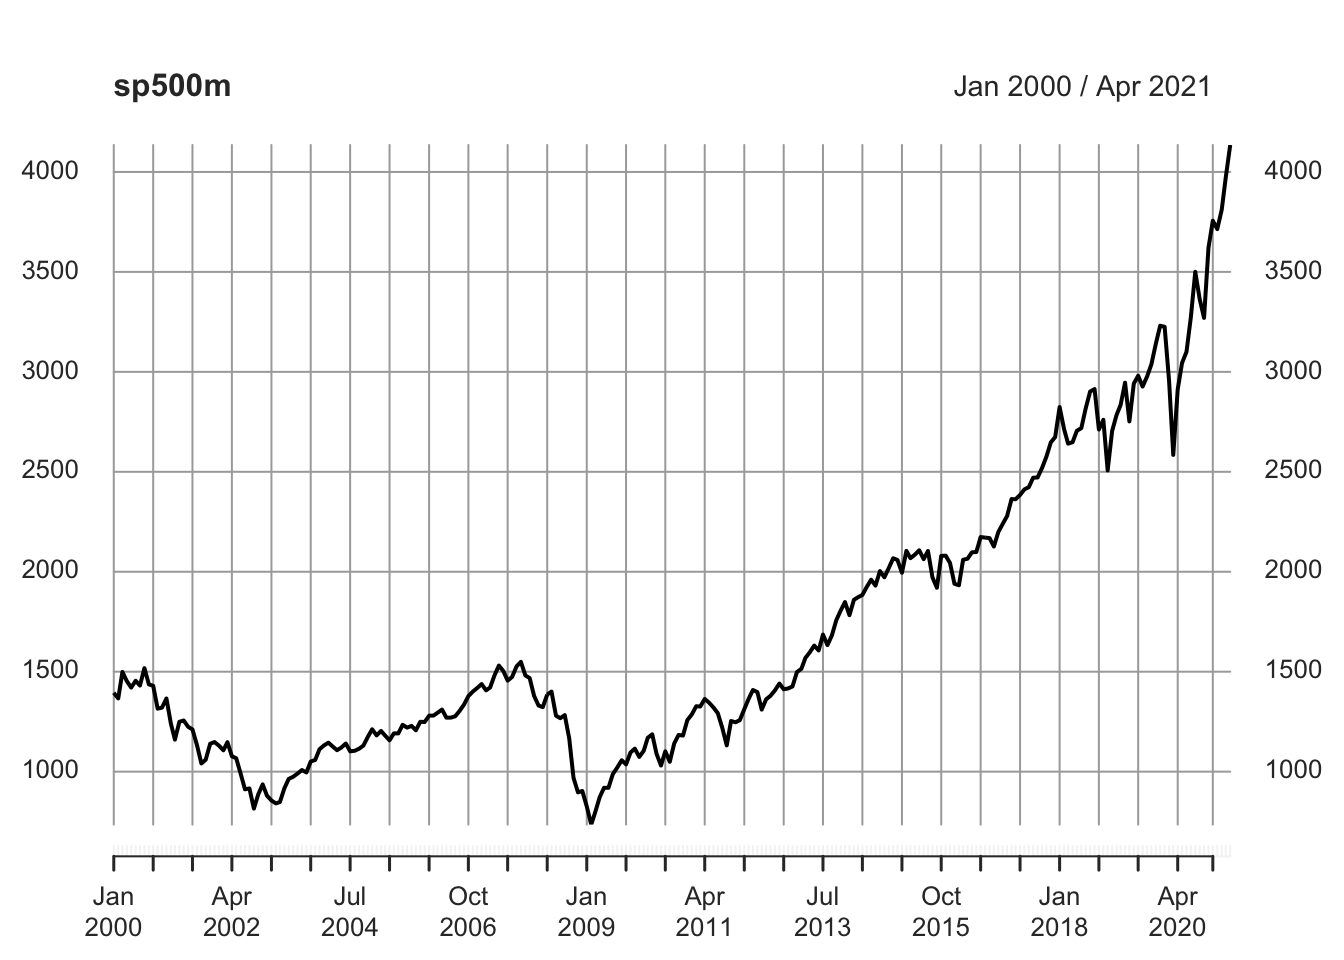
\includegraphics[width=0.9\textwidth]{../figuras-log/sp500m.png}
\caption{\label{fig:sp500m}Gráfica de la serie \texttt{sp500m}, correspondiente a la serie \texttt{sp500} convertida a datos de frecuencia mensual.}
\end{figure}

Aunque la serie con frecuencia mensual muestra claramente una tendencia (no estacionariedad), se lleva a cabo la prueba aumentada de Dickey-Fuller para probarla formalmente. Se obtiene un valor del estadístico de 0.24955, y un valor $p$ correspondiente de 0.99, lo cual indica que no se puede rechazar la hipótesis nula de que la serie \texttt{sp500m} presenta raíz unitaria y es por tanto no estacionaria.

Para obtener una serie estacionaria se calculan las primeras diferencias logarímicas y se almacenan en una nueva serie llamada \texttt{sp500m-1}. La figura (\ref{fig:sp500m-1}) muestra la gráfica de esta serie.

\begin{figure}[H]
\centering
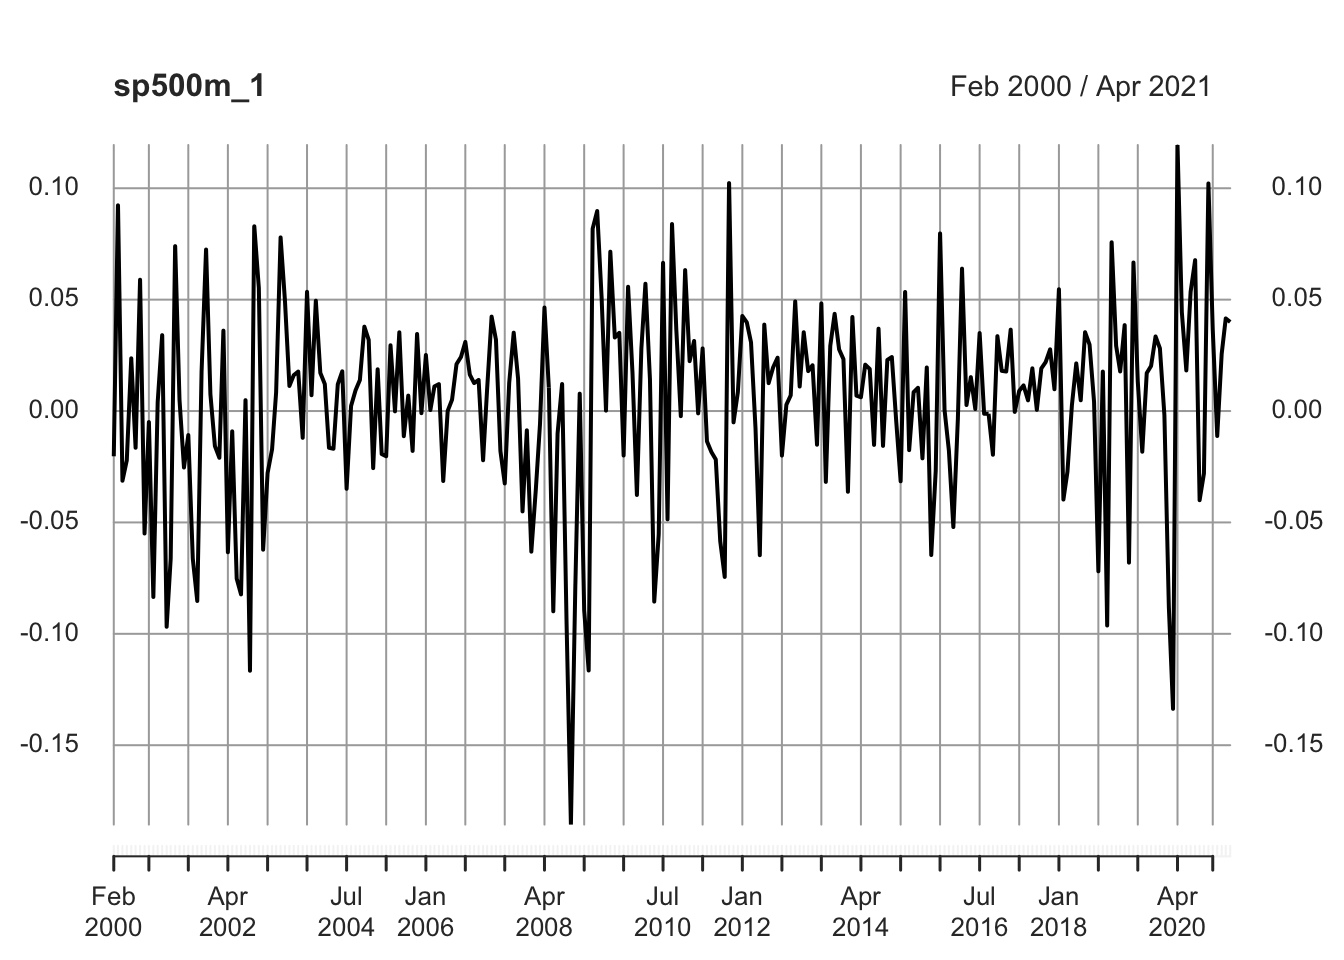
\includegraphics[width=0.9\textwidth]{../figuras-log/sp500m_1.png}
\caption{\label{fig:sp500m-1}Gráfica de la serie \texttt{sp500m-1}, correspondiente a las primeras diferencias logarítmicas de la serie \texttt{sp500m}.}
\end{figure}

Al llevar a cabo la prueba aumentada de Dickey-Fuller sobre la serie \texttt{sp500m-1}, se obtiene un valor del estadístico igual a -5.6307, y un valor $p$ de 0.01, por lo cual se rechaza la hipótesis nula de que la serie \texttt{sp500m-1} tiene raíz unitaria, con un nivel de significancia $\alpha=0.05$.

Con esta nueva serie se repite  el procedimiento de búsqueda del modelo $\mathrm{ARMA}(p, q)$ óptimo, esta vez variando independientemente los parámetros $p$ y $q$ entre 1 y 10. Los criterios de información de Akaike (AIC) para cada modelo estimado son los siguientes:

\begin{table}[H]
\centering
\begin{tabularx}{0.9\textwidth}{YYYYYY}
\toprule
\multirow{2}{*}{$p$} & \multicolumn{5}{c}{$q$} \\
\cmidrule{2-6}
& 1 & 2 & 3 & 4 & 5 \\
%\midrule
1 & -867.2541&-865.3633&-864.71&-862.7104&-861.8807 \\
2 & -865.3693&-863.3677&-862.7102&-864.6792&-866.0731 \\
3 & -864.6408&-866.7266&-860.7138&-862.9615&-864.1541 \\
4 & -862.711&-864.7479&-863.3447&-866.093&-864.2054 \\
5 & -862.2362&-865.7666&-865.8954&-864.2013&-862.1549 \\
6 & -861.5606&-863.7697&-861.8072&-859.7982&-858.1328 \\
7 & -860.716&-861.5805&-859.8537&-860.7448&-860.7414 \\
8 & -859.7129&-860.6694&-858.0276&-858.8732&-858.1847 \\
9 & -858.6157&-856.6158&-854.6661&-859.8558&-857.7075 \\
10 & -856.6165&-854.6157&-856.795&-855.3184&-854.8144 \\
\midrule
\multirow{2}{*}{$p$} & \multicolumn{5}{c}{$q$} \\
\cmidrule{2-6}
& 6 & 7 & 8 & 9 & 10 \\
1 & -860.7557&-859.5645&-859.6983&-859.3776&-857.9054 \\
2 & -864.1559&-861.7982&-860.6344&-858.666&-864.0275 \\
3 & -862.1545&-860.1897&-858.2261&-856.6941&-861.3563 \\
4 & -860.1826&-863.0429&-860.0398&-854.6932&-854.4539 \\
5 & -858.212&-857.1438&-858.3866&-857.857&-855.7522 \\
6 & -856.1995&-860.2383&-860.4172&-860.8915&-858.9088 \\
7 & -859.1952&-862.6002&-857.2897&-858.8627&-856.9329 \\
8 & -862.6773&-855.7247&-857.2197&-857.0902&-855.2309 \\
9 & -860.8289&-858.8275&-857.1309&-857.057&-856.0372 \\
10 & -858.8293&-856.2785&-854.71&-855.846&-859.5798 \\
%\midrule
\bottomrule
\end{tabularx}
\caption{\label{tab:akaike-m}Valores del criterio de información de Akaike (AIC) para el modelo $\mathrm{ARMA}(p, q)$, donde el valor de $p$ es el número de fila y el valor de $q$ es el número de columna, para la serie \texttt{sp500m-1}.}
\end{table}

Como se puede observar en  el cuadro (\ref{tab:akaike-m}), el valor mínimo del criterio de información AIC es -867.2541 y corresponde al modelo de orden $p=1$, $q=1$, por lo que el modelo óptimo es $\mathrm{ARMA}(1, 1)$. Al estimarlo se obtienen los siguientes coeficientes:

\begin{table}[H]
\centering
\begin{tabularx}{0.6\textwidth}{XYY}
\toprule
Coeficiente & Valor & Error estándar \\
\midrule
\texttt{ar1} & -0.6531 & 0.2674 \\
\texttt{ma1} & -0.7552 & 0.2323 \\
\texttt{Media} & 0.0043 & 0.0029 \\
\bottomrule
\end{tabularx}
\caption{\label{tab:arma-m-1-1}Coeficientes de la estimación del modelo ARMA(1, 1), para la serie \texttt{sp500m-1}. Los valores entre paréntesis son errores estándar.}
\end{table}

A este modelo le corresponde una $\sigma^2$ estimada de 0.001914, un valor de log-likelihood de 437.63, y los siguientes valores de criterios de información:
\begin{itemize}
\item Criterio de información de Akaike (AIC): -867.25.
\item Criterio de información bayesiano (BIC): -853.09.
\end{itemize}

Para verificar si en este caso el modelo es adecuado, se evalúa si los residuales del modelo estimado son ruido blanco. La figura (\ref{fig:residuales-m}) muestra la gráfica de los mismos, así como su función de autocorrelación y su histograma de frecuencias. Se observa que la gráfica parece ser estacionaria alrededor de la media cero, lo cual indica que no tienen tendencia. Además, no existe autocorrelación significativa y parecen distribuirse normalmente con media cero. Esto sugiere que efectivamente se comportan como ruido blanco.

Se llevó a cabo la prueba de Ljung-Box sobre los residuales del modelo ajustado, obteniendo un valor del estadístico $Q^* = 22.279$ para 24 rezagos, que equivale a un valor $p$ de 0.3836, por lo que se rechaza la hipótesis nula de que los residuales presentan autocorrelación conjunta, con un nivel de significancia $\alpha = 0.05$.

Como resultado de este análisis, se puede concluir que los residuales del modelo estimado se comportan como ruido blanco, lo cual indica que el modelo captura adecuadamente la información de la serie de tiempo, y no es necesario por lo tanto buscar una especificación más compleja. La especificación del modelo ARMA sobre la serie \texttt{sp500m-1}, que corresponde a las observaciones de la serie original \texttt{sp500-1} con frecuencia mensual, es la siguiente:
\[ y_t = 0.0043 -0.6531 y_{t-1} + 0.7552 + e_t \]

\begin{figure}[H]
\centering
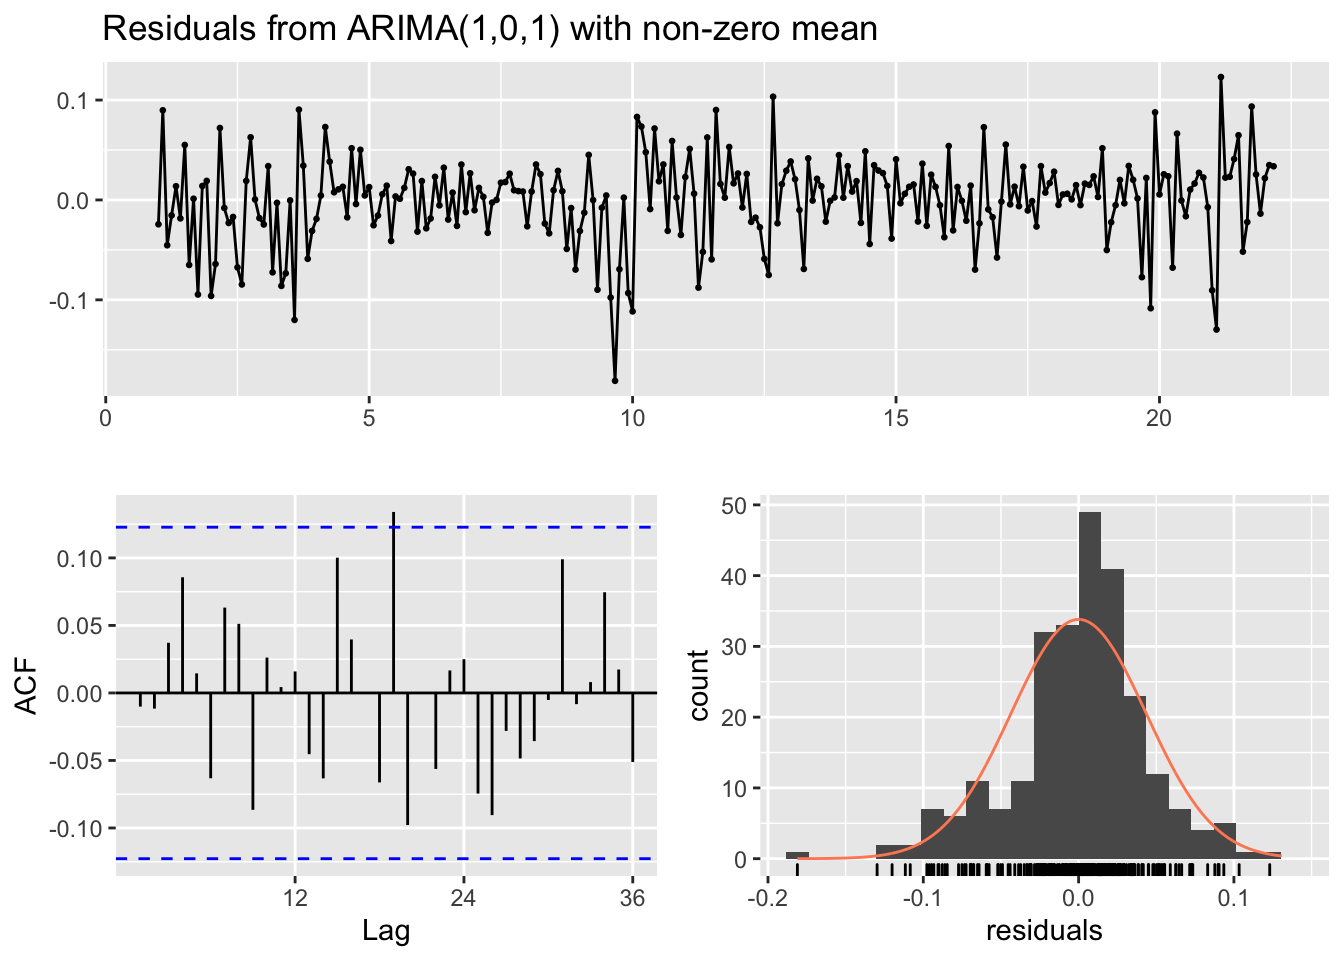
\includegraphics[width=0.9\textwidth]{../figuras-log/residuales_m.png}
\caption{\label{fig:residuales-m}Gráfica de los residuales del modelo $\mathrm{ARMA(7, 7)}$, su autocorrelación y su histograma, para la serie \texttt{sp500m-1}.}
\end{figure}

Finalmente, se generaron pronósticos dentro y fuera de la muestra, utilizando como serie de ajuste (\emph{training set}) las observaciones hasta el 31 de diciembre de 2018, y como serie de evaluación las observaciones a partir del 1 de enero de 2019. La figura (\ref{fig:pronosticos}) muestra estos pronósticos.

\begin{figure}[H]
\centering
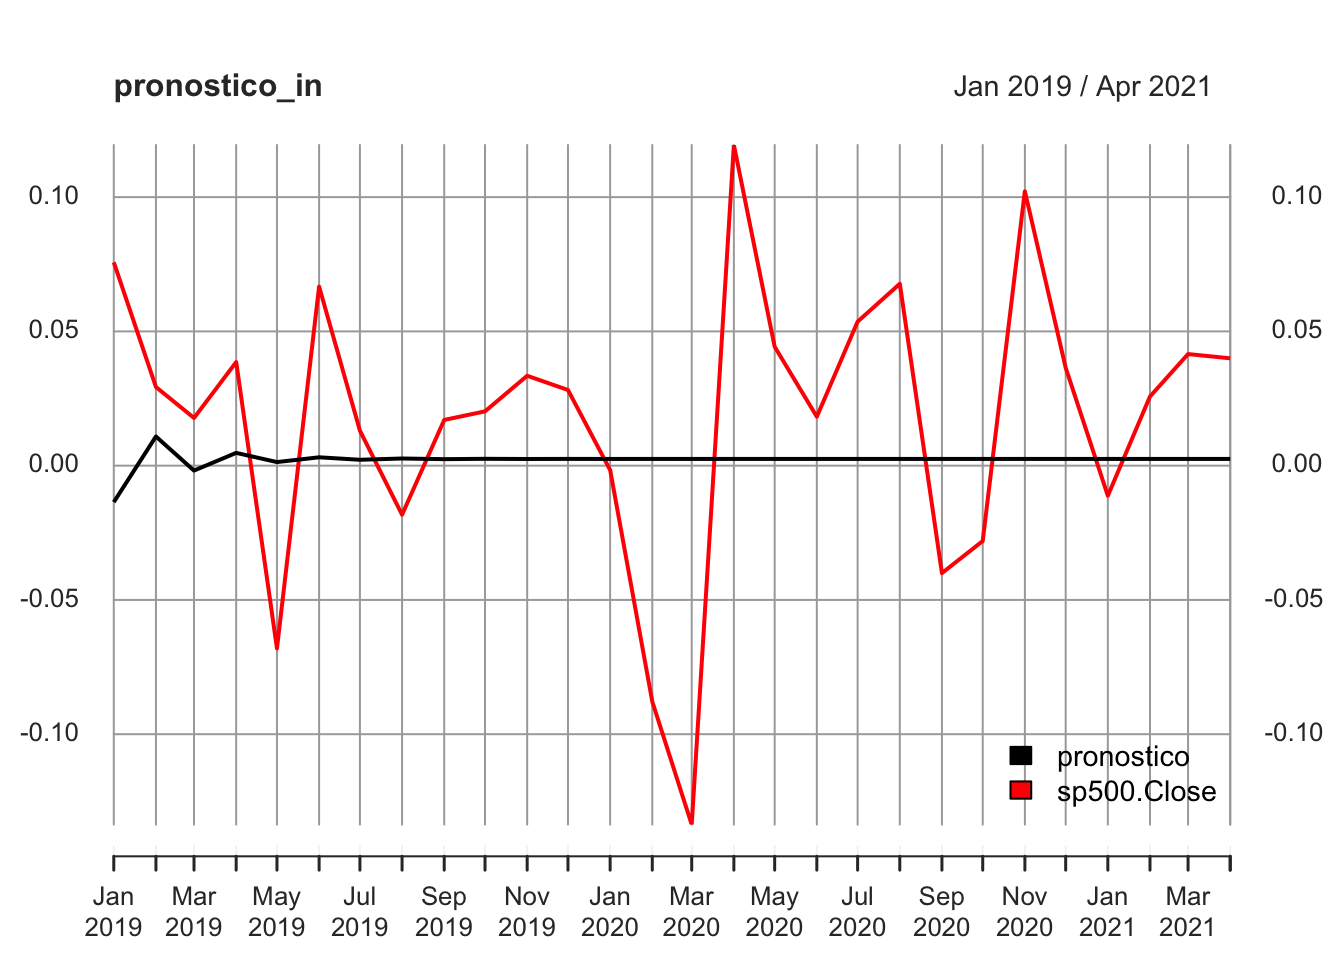
\includegraphics[width=0.7\textwidth]{../figuras-log/pronostico_in.png}
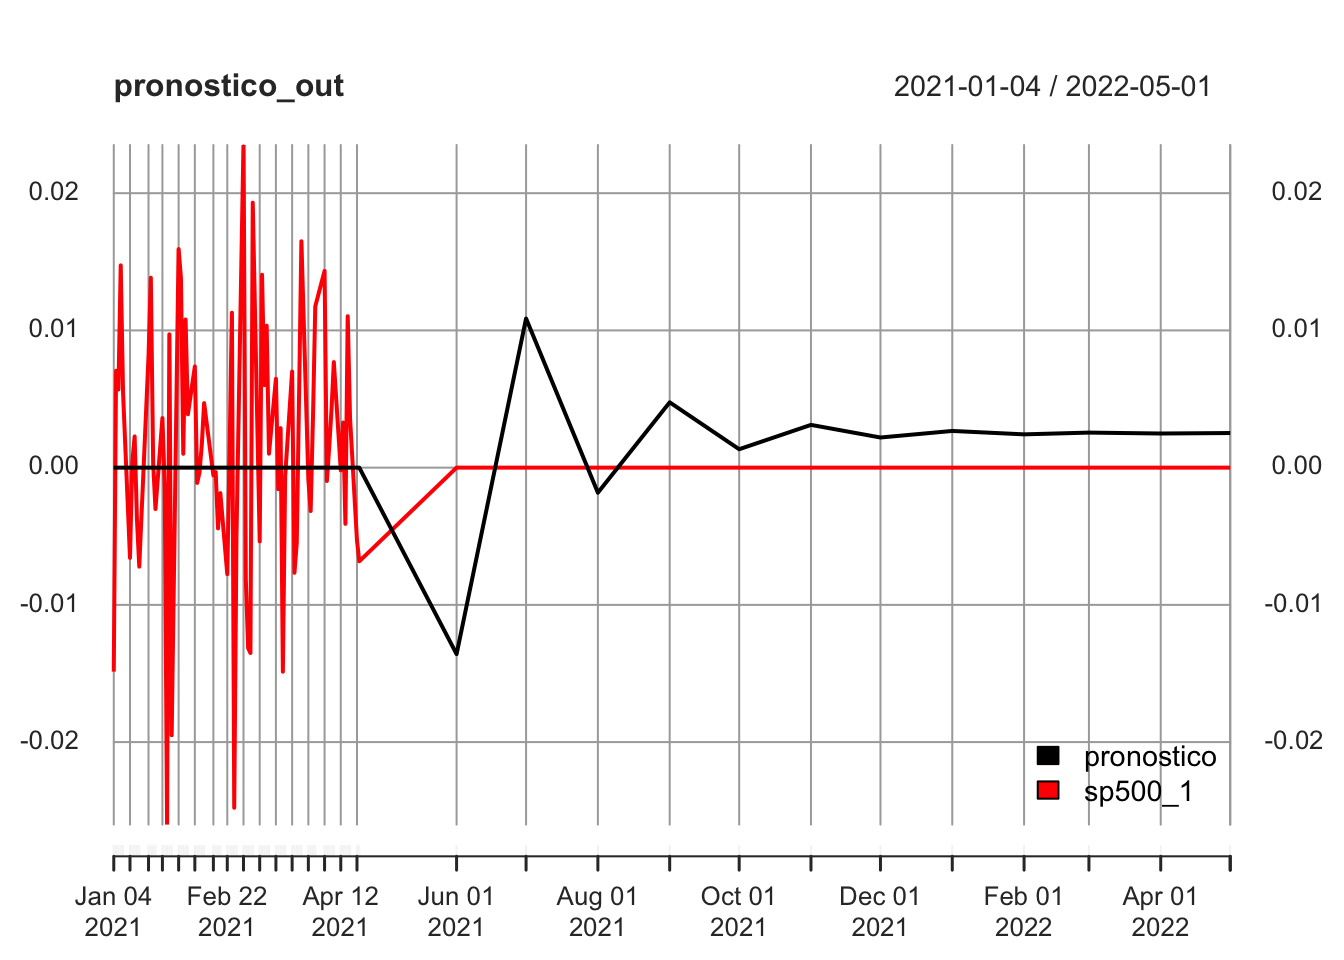
\includegraphics[width=0.7\textwidth]{../figuras-log/pronostico_out.png}
\caption{\label{fig:pronosticos}Gráfica de los pronósticos dentro de la muestra (arriba) y fuera de la muestra (abajo) del modelo $\mathrm{ARMA(1, 1)}$ para la serie \texttt{sp500m-1}.}
\end{figure}

En la figura (\ref{fig:pronosticos}) se observa que los pronósticos decaen rápidamente a cero, debido al bajo orden de la especificación del modelo ARMA elegido.

Adicionalmente se calcularon algunas medidas de error para el pronóstico dentro de la muestra:

\begin{table}[H]
\centering
\begin{tabularx}{0.6\textwidth}{XY}
\toprule
Medida de error & Valor \\
\midrule
MAE & 4.49\% \\
MSE & 0.31\% \\
RMSE & 5.61\% \\
MAPE & 102.33 \% \\
\bottomrule
\end{tabularx}
\caption{\label{tab:medidas-error}Medidas del error de pronóstico.}
\end{table}


\newpage
\section{Modelo de volatilidad GARCH}

A continuación se busca estimar un modelo de volatilidad de clase GARCH para la serie \texttt{sp500-1}. La forma general de un modelo $\mathrm{GARCH}(p, q)$ es la siguiente:
\[ \sigma^2_t =  \alpha_0 + \sum_{i=1}^q \alpha_i u^2_{t-i} + \sum_{j=1}^p \beta_j \sigma^2_{t-j} \]

La metodología para seleccionar el mejor modelo es análoga a la que se empleó para encontrar el modelo ARMA óptimo: se estimarán 25 modelos $\mathrm{GARCH}(p, q)$ diferentes, variando independientemente los parámetros $p$ y $q$ entre 1 y 5. Para cada modelo estimado se calculó el criterio de información bayesiano (BIC), y los resultados son los siguientes:

\begin{table}[H]
\centering
\begin{tabularx}{0.9\textwidth}{YYYYYY}
\toprule
\multirow{2}{*}{$p$} & \multicolumn{5}{c}{$q$} \\
\cmidrule{2-6}
& 1 & 2 & 3 & 4 & 5 \\
\midrule
1 & -6.449218&-6.446946&-6.443827&-6.44072&-6.437653 \\
2 & -6.449317&-6.446842&-6.443833&-6.440217&-6.437456 \\
3 & -6.445972&-6.443891&-6.440953&-6.439616&-6.434335 \\
4 & -6.442883&-6.440892&-6.437719&-6.43575&-6.43287 \\
5 & -6.439802&-6.437584&-6.438893&-6.432912&-6.430124 \\
\bottomrule
\end{tabularx}
\caption{\label{tab:bic}Valores del criterio de información bayesiano (BIC) para el modelo $\mathrm{GARCH}(p, q)$, donde el valor de $p$ es el número de fila y el valor de $q$ es el número de columna, para la serie \texttt{sp500-1}.}
\end{table}

Al analizar los resultados del criterio de información bayesiano presentados en el cuadro (\ref{tab:bic}), se observa que el valor mínimo es -6.449317, que corresponde a la parametrización $p=2$, $q=1$. Por lo tanto, la especificación de modelo de volatilidad GARCH óptima es $\mathrm{GARCH}(2, 1)$.

Al estimar este modelo se obtienen los siguientes resultados:

\begin{table}[H]
\centering
\begin{tabularx}{0.9\textwidth}{XXXXXX}
\toprule
Parámetro & Estimación & Error estándar & Estadístico $t$ & Valor $p$ \\
\midrule
\texttt{mu}&0.000621&0.000075&8.3143&0 \\
\texttt{ar1}&0.891415&0.014314&62.275&0 \\
\texttt{ar2}&0.043317&0.014708&2.9452&0.003228 \\
\texttt{ma1}&-0.95618&0.001249&-765.305&0 \\
\texttt{omega}&0.000003&0.000001&3.3912&0.000696 \\
\texttt{alpha1}&0.081623&0.013697&5.9591&0 \\
\texttt{alpha2}&0.064236&0.016971&3.7849&0.000154 \\
\texttt{beta1}&0.834458&0.012874&64.8185&0 \\
\bottomrule
\end{tabularx}
\caption{\label{tab:garch-2-1}Resultados de la estimación del modelo $\mathrm{GARCH}(2, 1)$ sobre la serie \texttt{sp500-1}.}
\end{table}

Este modelo tiene un log-likelihood de 17308.84, y los siguientes criterios de información:
\begin{itemize}
\item Akaike: -6.4592.
\item Bayes: -6.4493.
\item Hannan-Quinn: -6.4557.
\end{itemize}

Además, al analizar los valores $p$ mostrados en el cuadro (\ref{tab:garch-2-1}) se observa que todos los coeficientes son significativos con un nivel de significancia $\alpha=0.05$.

Cabe preguntarse qué sucede al aumentar el orden del modelo a $p=3$, $q=2$, para evaluar si es capaz de ajustarse mejor a los datos. Al estimar el modelo $\mathrm{GARCH}(3, 2)$ se obtienen los siguientes resultados:

\begin{table}[H]
\centering
\begin{tabularx}{0.9\textwidth}{XXXXXX}
\toprule
Parámetro & Estimación & Error estándar & Estadístico $t$ & Valor $p$ \\
\midrule
\texttt{mu}&0.000621&0.000072&8.56391&0\\
\texttt{ar1}&0.594759&0.014221&41.82339&0\\
\texttt{ar2}&0.30497&0.016806&18.14609&0\\
\texttt{ar3}&0.016698&0.014684&1.13714&0.255482\\
\texttt{ma1}&-0.659325&0.001306&-504.96046&0\\
\texttt{ma2}&-0.28514&0.003228&-88.34446&0\\
\texttt{omega}&0.000005&0.000001&3.99799&0.000064\\
\texttt{alpha1}&0.079003&0.013758&5.74248&0\\
\texttt{alpha2}&0.143467&0.01355&10.58773&0\\
\texttt{alpha3}&0.025565&0.017609&1.45182&0.146552\\
\texttt{beta1}&0.069598&0.092797&0.75001&0.453251\\
\texttt{beta2}&0.649545&0.087091&7.45821&0\\
\bottomrule
\end{tabularx}
\caption{\label{tab:garch-3-2}Resultados de la estimación del modelo $\mathrm{GARCH}(3, 2)$ sobre la serie \texttt{sp500-1}.}
\end{table}

Este modelo tiene un log-likelihood de 17,311.48, y los siguientes valores para los criterios de información:
\begin{itemize}
\item Akaike: -6.4586.
\item Bayes: -6.4439.
\item Hannan-Quinn: -6.4535.
\end{itemize}

Al observar en el cuadro (\ref{tab:garch-3-2}) los valores $p$ de los coeficientes, se observa que $\alpha_3$ y $\beta_1$ no son significativos. Por este motivo, conservamos la especificación original $\mathrm{GARCH(2, 1)}$.

Así, el modelo de volatilidad elegido es una especificación $\mathrm{GARCH}(2, 1)$ que tiene la siguiente forma:
\[ \sigma^2_t = 0.0006 + 0.0816 u^2_{t-1} + 0.0642 u^2_{t-2} + 0.8345 \sigma^2_{t-1} \]

Resta verificar si los residuales se comportan como ruido blanco. La figura (\ref{fig:garch-2-1-residuales}) muestra la gráfica de normalidad (QQ plot) y de autocorrelación de los residuales del modelo estimado. Se observa que si bien los residuales parecen alejarse de la normalidad en los valores extremos, en general se ajustan bien a una distribución normal, y además no presentan autocorrelación significativa (los coeficientes de autocorrelación se encuentran dentro de las bandas de 95\% de confianza, lo que indica que con un nivel de significancia de $\alpha=0.05$, la autocorrelación conjunta de los residuales es cero).

\begin{figure}[H]
\centering
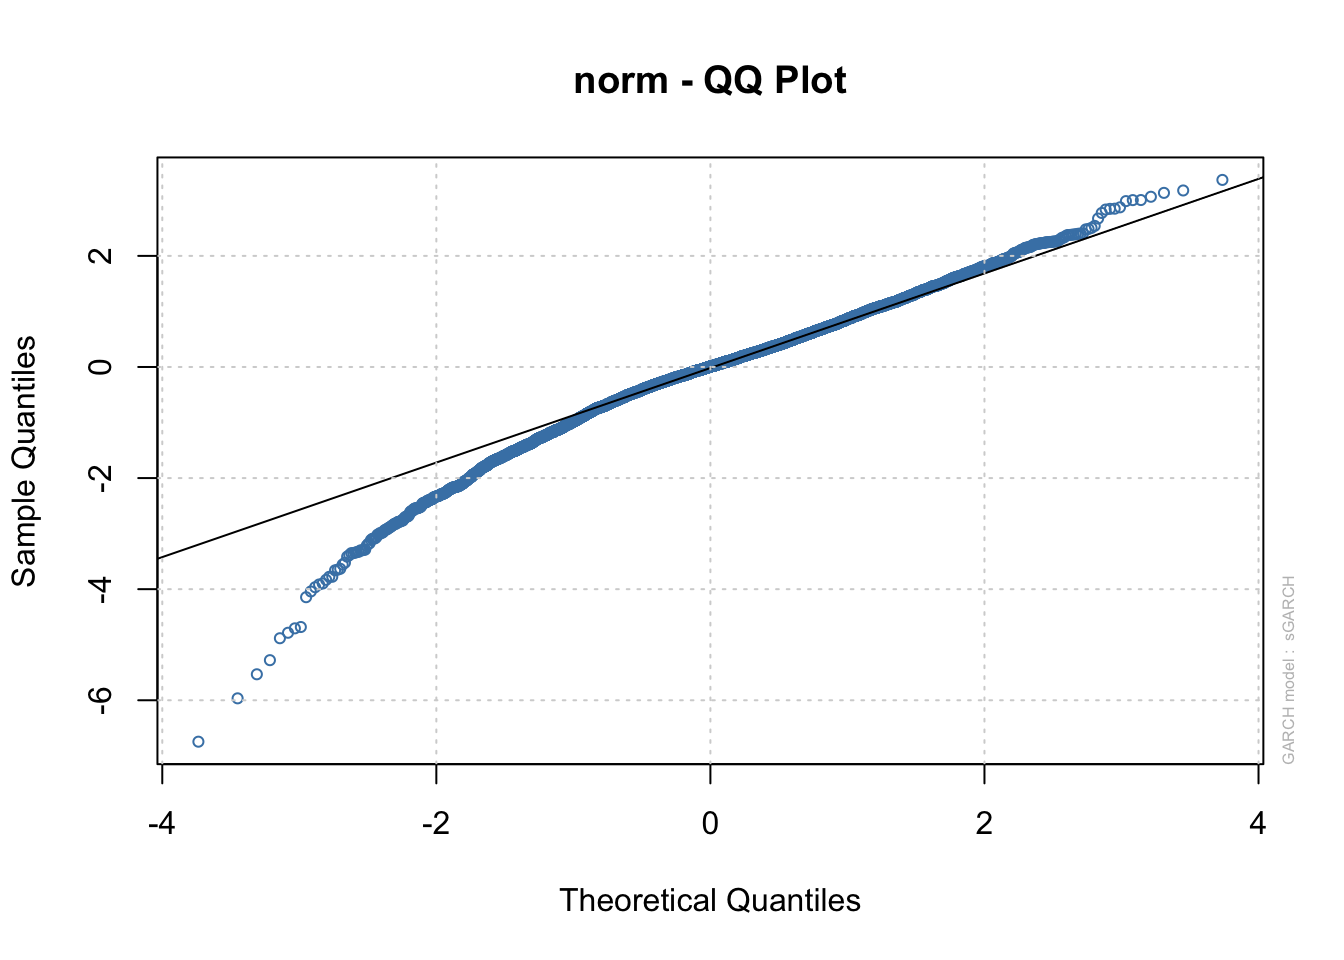
\includegraphics[width=0.7\textwidth]{../figuras-log/garch_2_1_qq.png}
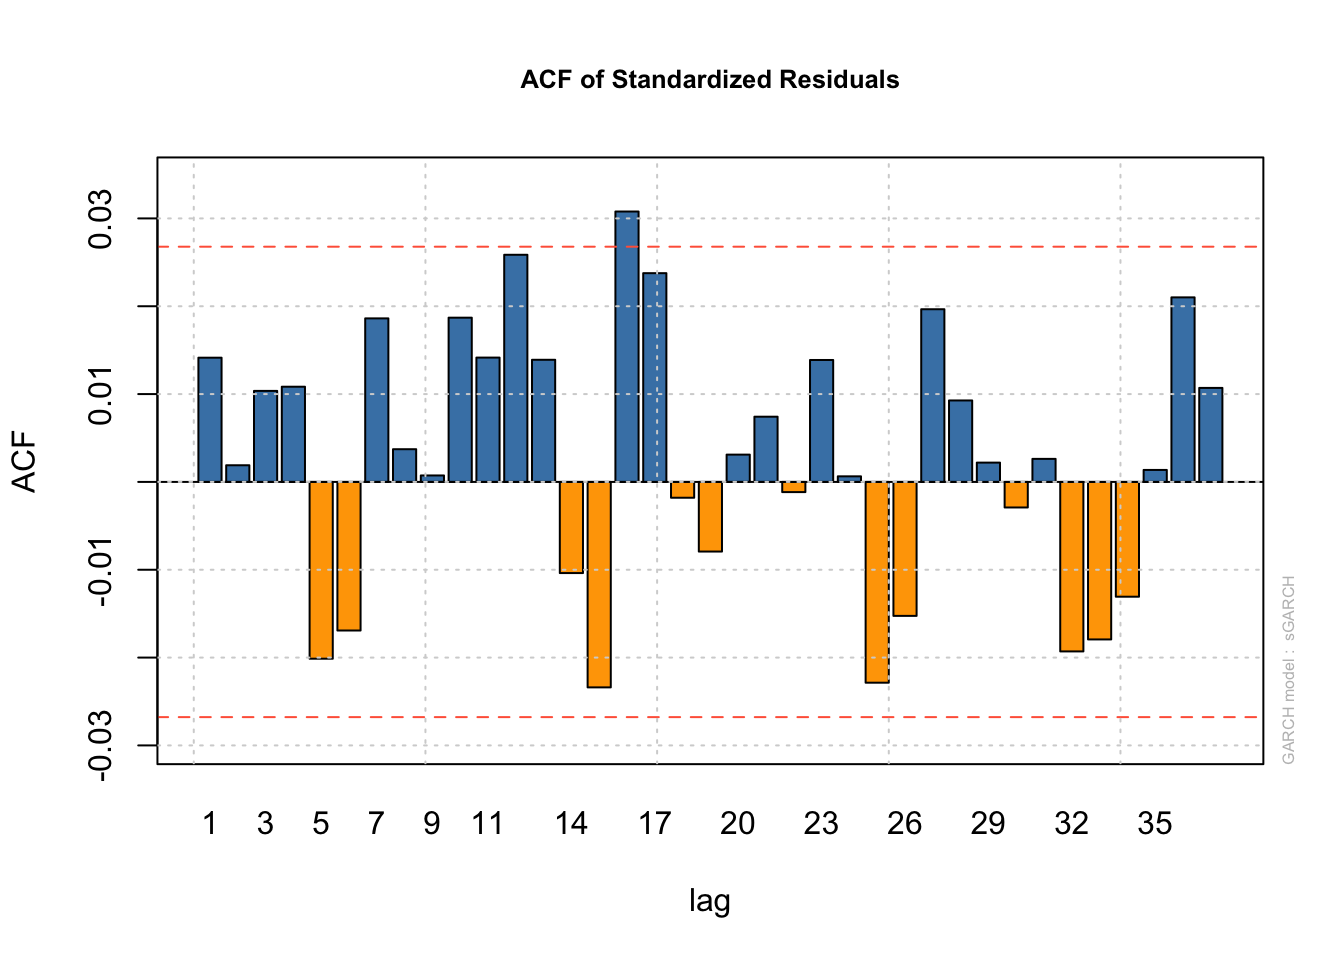
\includegraphics[width=0.7\textwidth]{../figuras-log/garch_2_1_autocorrelacionresiduales.png}
\caption{\label{fig:garch-2-1-residuales}Gráfica de normalidad (QQ plot) (arriba) y de autocorrelación (abajo) de los residuales del modelo $\mathrm{GARCH(2, 1)}$ para la serie \texttt{sp500-1}.}
\end{figure}

Además, en la figura (\ref{fig:garch-2-1-volatilidad}) se muestra la volatilidad de la serie con bandas de 2 desviaciones estándar de acuerdo a la volatilidad estimada. Se observa que el modelo GARCH propuesto estima adecuadamente la volatilidad de la serie.

\begin{figure}[H]
\centering
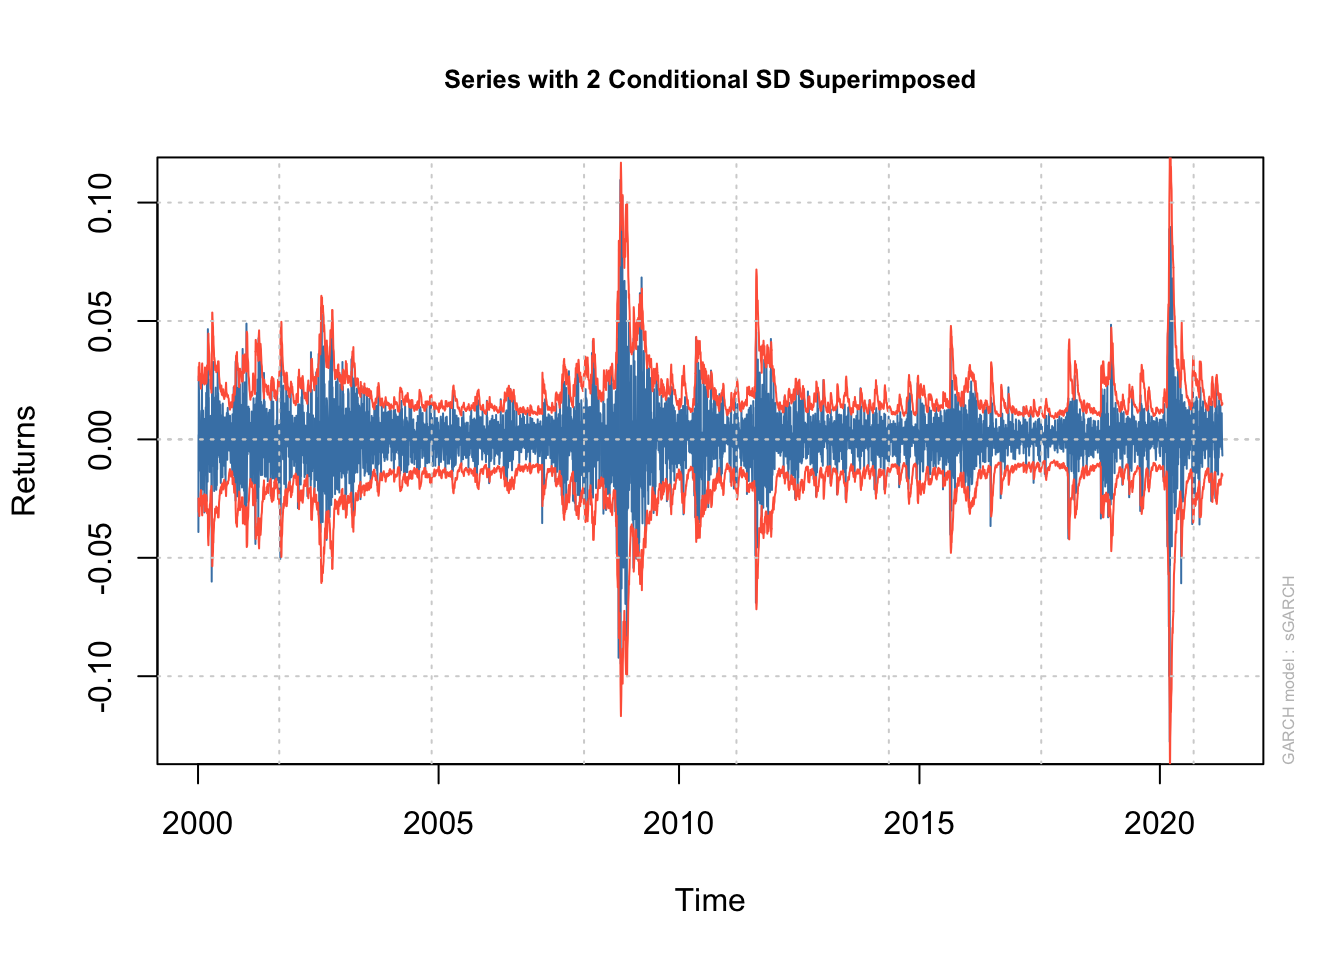
\includegraphics[width=0.9\textwidth]{../figuras-log/garch_2_1_volatilidad.png}
\caption{\label{fig:garch-2-1-volatilidad}Gráfica de volatilidad estimada ($\pm 2\sigma$) mediante el modelo $\mathrm{GARCH}(2,1)$ para la serie \texttt{sp500-1}.}
\end{figure}

Finalmente, se desea calcular el valor en riesgo de la serie ($\mathrm{VaR}_p$), para valores de $p$ (probabilidades de pérdida) de 0.10, 0.05 y 0.01. Se emplea el método histórico, que consiste en calcular el valor en riesgo con probabilidad $p$ como el valor absoluto del percentil $1-p$. Así, se obtienen los siguientes resultados:

\begin{table}[H]
\centering
\begin{tabularx}{0.6\textwidth}{YY}
\toprule
Probabilidad $p$ & Valor en riesgo ($\mathrm{VaR}_p$) \\
\midrule
0.10 & 1.3012\% \\
0.05 & 1.9132\% \\
0.01 & 3.5206\% \\
\bottomrule
\end{tabularx}
\caption{\label{tab:var}Valor en riesgo calculado para $p=0.90, 0.95, 0.99$ para los retornos de la serie \texttt{sp500}.}
\end{table}

Esto se interpreta de la siguiente forma: con probabilidad de 10\% se puede observar una pérdida (en un día) de 1.3\%, mientras que con probabilidad de 5\% la pérdida puede ser de 1.9\%, y con probabilidad de 1\% puede llegar a ser de 3.5\%.


\newpage
\section{Modelo de vectores autorregresivos}

Finalmente, se estimará un modelo de vectores autorregresivos (VAR). Para ello se emplea, además de la serie ya presentada \texttt{sp500}, una serie que contiene el retorno de los bonos de largo plazo (10 años) del Tesoro de EUA. El objetivo es determinar si las variaciones de una serie afectan a la otra. La figura (\ref{fig:ltc}) presenta la gráfica de esta serie de tiempo.

\begin{figure}[H]
\centering
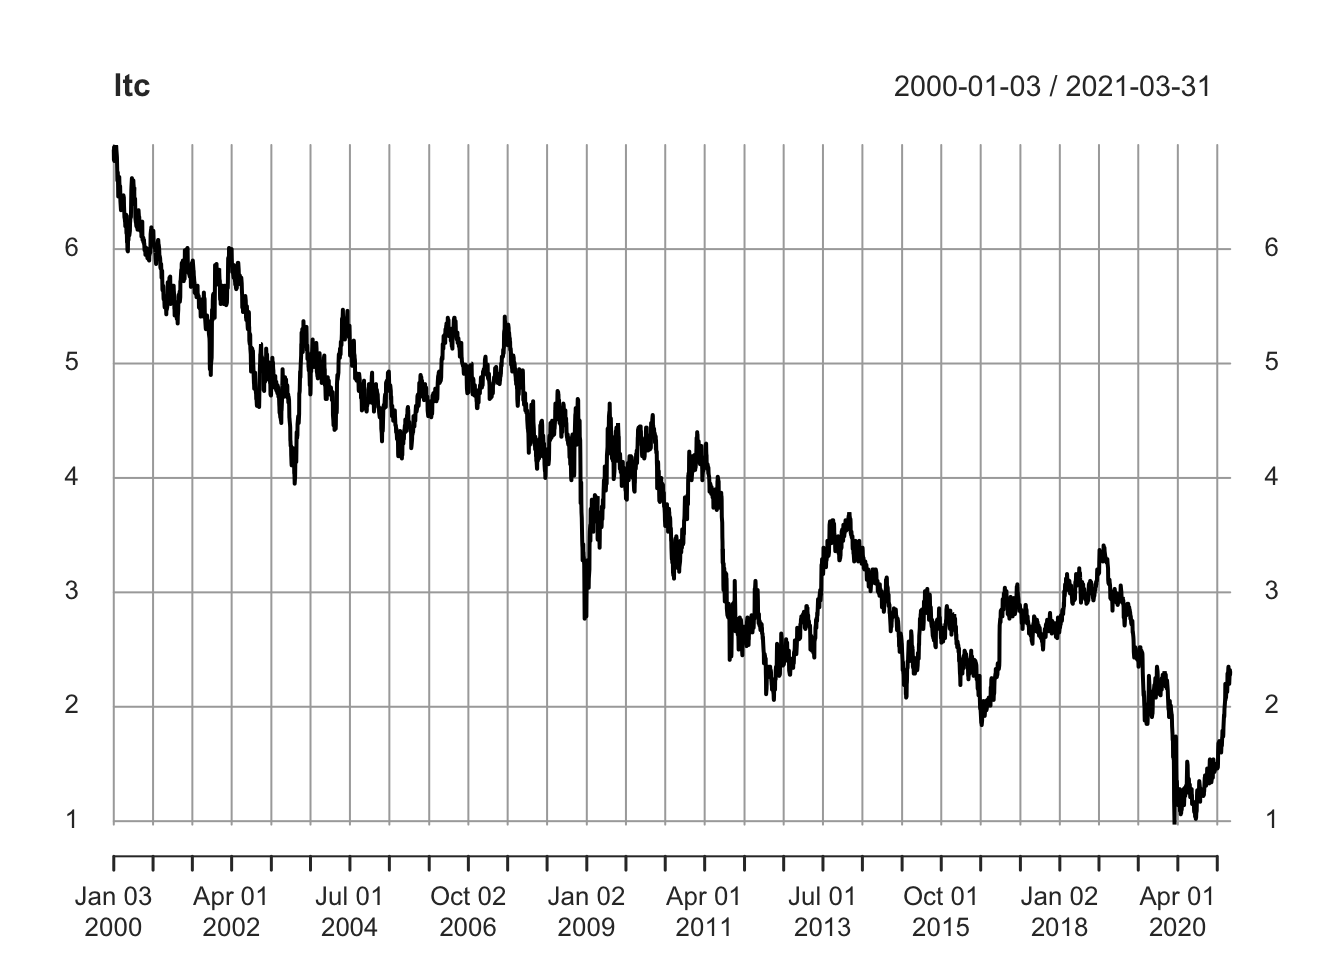
\includegraphics[width=0.9\textwidth]{../figuras-log/ltc.png}
\caption{\label{fig:ltc}Gráfica de la serie \texttt{ltc}, que representa el retorno de los bonos de largo plazo (10 años) del Tesoro estadounidense.}
\end{figure}

Para la estimación de modelos VAR, \texttt{R} dispone de una función que permite seleccionar automáticamente el número óptimo de rezagos. La tabla (\ref{tab:var-select}) muestra los criterios de información de Akaike (AIC) y Hannan-Quinn (HQ) para rezagos del 1 al 10. Se observa que el número óptimo es 10.

\begin{table}[H]
\centering
\begin{tabularx}{0.6\textwidth}{YYY}
\toprule
Rezagos & AIC & HQ \\
\midrule
1&0.1771518&0.1797549\\
2&0.1528343&0.1571728\\
3&0.1477548&0.1538286\\
4&0.1478244&0.1556336\\
5&0.146091&0.1556355\\
6&0.1473937&0.1586736\\
7&0.1343622&0.1473775\\
8&0.1229181&0.1376687\\
9&0.1187283&0.1352143\\
10&0.1129452&0.1311666\\
\bottomrule
\end{tabularx}
\caption{\label{tab:var-select}Criterios de información de acuerdo al número de rezagos (1 a 10).}
\end{table}

Se estima el modelo y se obtienen los siguientes resultados para los coeficientes de la ecuación de \texttt{sp500}:

\begin{table}[H]
\centering
\begin{tabularx}{0.9\textwidth}{XXXXX}
\toprule
Variable & Valor & Error estándar & Estadístico $t$ & Valor $p$ \\
\midrule
sp500.l1&0.87675&0.01448&60.543& $<$ 2e-16 ***\\
ltc.l1&-1.87876&5.44382&-0.345&0.73002\\
sp500.l2&0.17905&0.01933&9.261& $<$ 2e-16 ***\\
ltc.l2&-9.2554&7.72063&-1.199&0.230664\\
sp500.l3&-0.02093&0.01935&-1.081&0.279546\\
ltc.l3&7.64278&7.71843&0.99&0.322122\\
sp500.l4&-0.08706&0.01915&-4.545&5.61e-06 ***\\
ltc.l4&3.69813&7.71172&0.48&0.631569\\
sp500.l5&0.04667&0.01914&2.439&0.014778 *\\
ltc.l5&-4.34354&7.70504&-0.564&0.572964\\
sp500.l6&-0.09209&0.01915&-4.81&1.55e-06 ***\\
ltc.l6&16.75382&7.70438&2.175&0.029706 *\\
sp500.l7&0.19857&0.01916&10.366& $<$ 2e-16 ***\\
ltc.l7&-28.9444&7.70762&-3.755&0.000175 ***\\
sp500.l8&-0.15877&0.01939&-8.19&3.24e-16 ***\\
ltc.l8&18.66746&7.71211&2.421&0.015531 *\\
sp500.l9&0.14443&0.01936&7.46&1.01e-13 ***\\
ltc.l9&-6.24425&7.71494&-0.809&0.418338\\
sp500.l10&-0.08713&0.0145&-6.011&1.97e-09 ***\\
ltc.l10&2.99994&5.43673&0.552&0.581115\\
const&4.75519&1.98274&2.398&0.016506 *\\
\bottomrule
\end{tabularx}
\caption{\label{tab:var-sp500}Coeficientes de la estimación de la ecuación de \texttt{sp500} en el modelo VAR. Códigos de significancia: *** = 0, ** = 0.001, * = 0.05, . = 0.1, vacío = 1.}
\end{table}

Mientras que para la ecuación de \texttt{ltc} los coeficientes son:

\begin{table}[H]
\centering
\begin{tabularx}{0.9\textwidth}{XXXXX}
\toprule
Variable & Valor & Error estándar & Estadístico $t$ & Valor $p$ \\
\midrule
sp500.l1&-0.0001181&0.00003864&-3.057&0.00225 **\\
ltc.l1&1.005&0.01453&69.183& $<$ 2e-16 ***\\
sp500.l2&0.0001292&0.00005159&2.504&0.01230 *\\
ltc.l2&-0.05484&0.0206&-2.662&0.00779 **\\
sp500.l3&-0.00004919&0.00005164&-0.952&0.34089\\
ltc.l3&0.04448&0.0206&2.16&0.03085 *\\
sp500.l4&-0.00004633&0.00005111&-0.906&0.36471\\
ltc.l4&0.0007148&0.02058&0.035&0.97229\\
sp500.l5&0.00008841&0.00005107&1.731&0.08347 .\\
ltc.l5&-0.001864&0.02056&-0.091&0.92778\\
sp500.l6&0.00003611&0.00005109&0.707&0.47967\\
ltc.l6&0.005426&0.02056&0.264&0.79186\\
sp500.l7&-0.00002949&0.00005112&-0.577&0.56408\\
ltc.l7&0.001737&0.02057&0.084&0.93271\\
sp500.l8&-0.00001946&0.00005173&-0.376&0.7068\\
ltc.l8&-0.03623&0.02058&-1.761&0.07835 .\\
sp500.l9&0.0001025&0.00005166&1.984&0.04730 *\\
ltc.l9&0.03062&0.02059&1.487&0.13703\\
sp500.l10&-0.00009559&0.00003868&-2.471&0.01349 *\\
ltc.l10&0.002915&0.01451&0.201&0.84076\\
const&0.01021&0.005291&1.931&0.05359 .\\
\bottomrule
\end{tabularx}
\caption{\label{tab:var-ltc}Coeficientes de la estimación de la ecuación de \texttt{ltc} en el modelo VAR. Códigos de significancia: *** = 0, ** = 0.001, * = 0.05, . = 0.1, vacío = 1.}
\end{table}

Por otra parte, la figura (\ref{fig:residuales-var}) muestra el análisis de residuales de ambas ecuaciones. Se observa que ambas series de residuales parecen ser estacionarias y no tener autocorrelación, lo cual sugiere que se comportan como ruido blanco.

\begin{figure}[H]
\centering
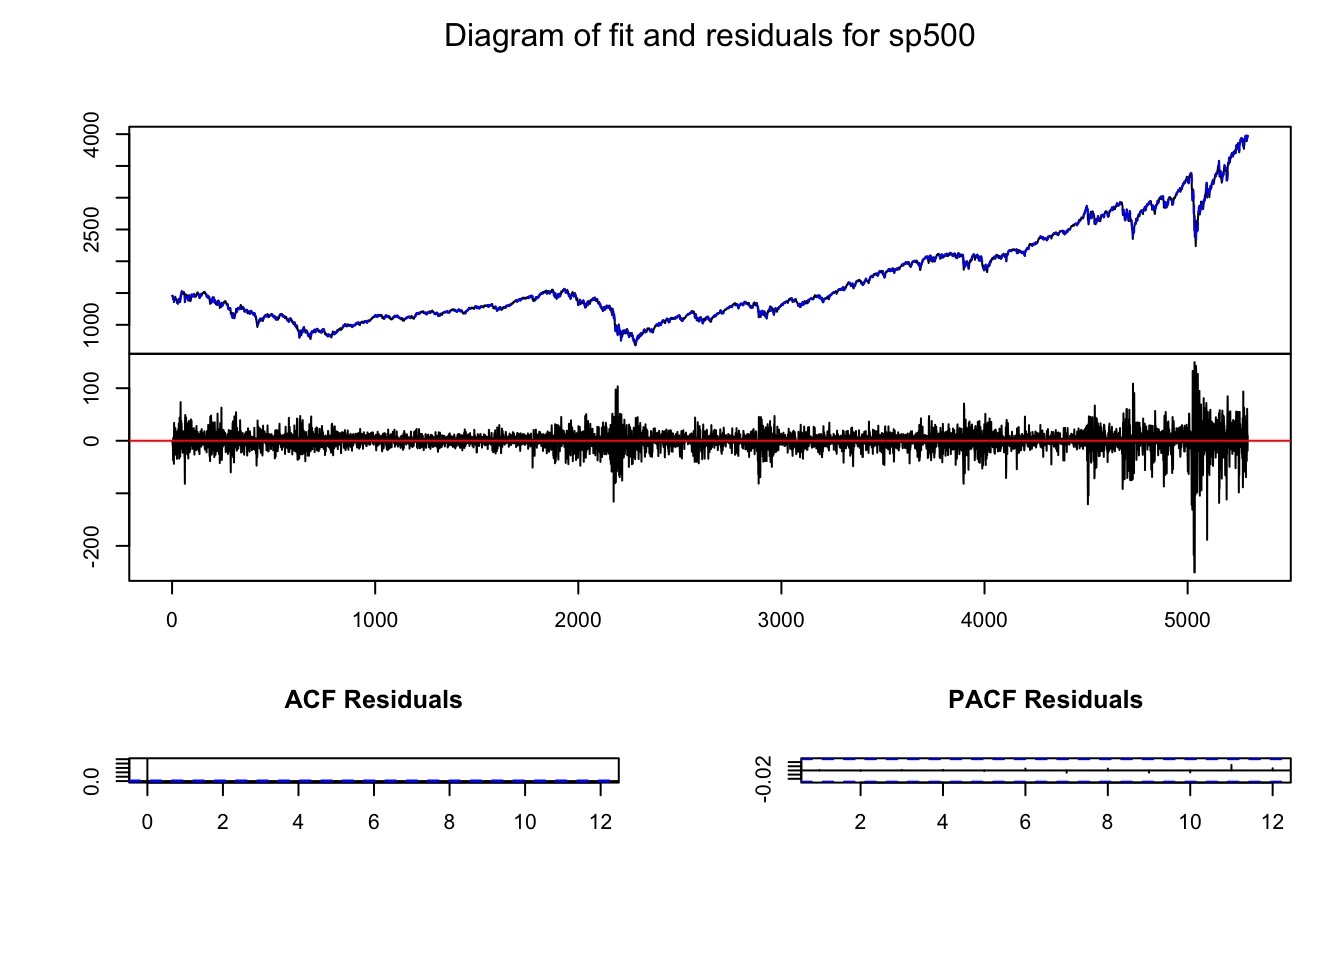
\includegraphics[width=0.8\textwidth]{../figuras-log/var-sp500.png}
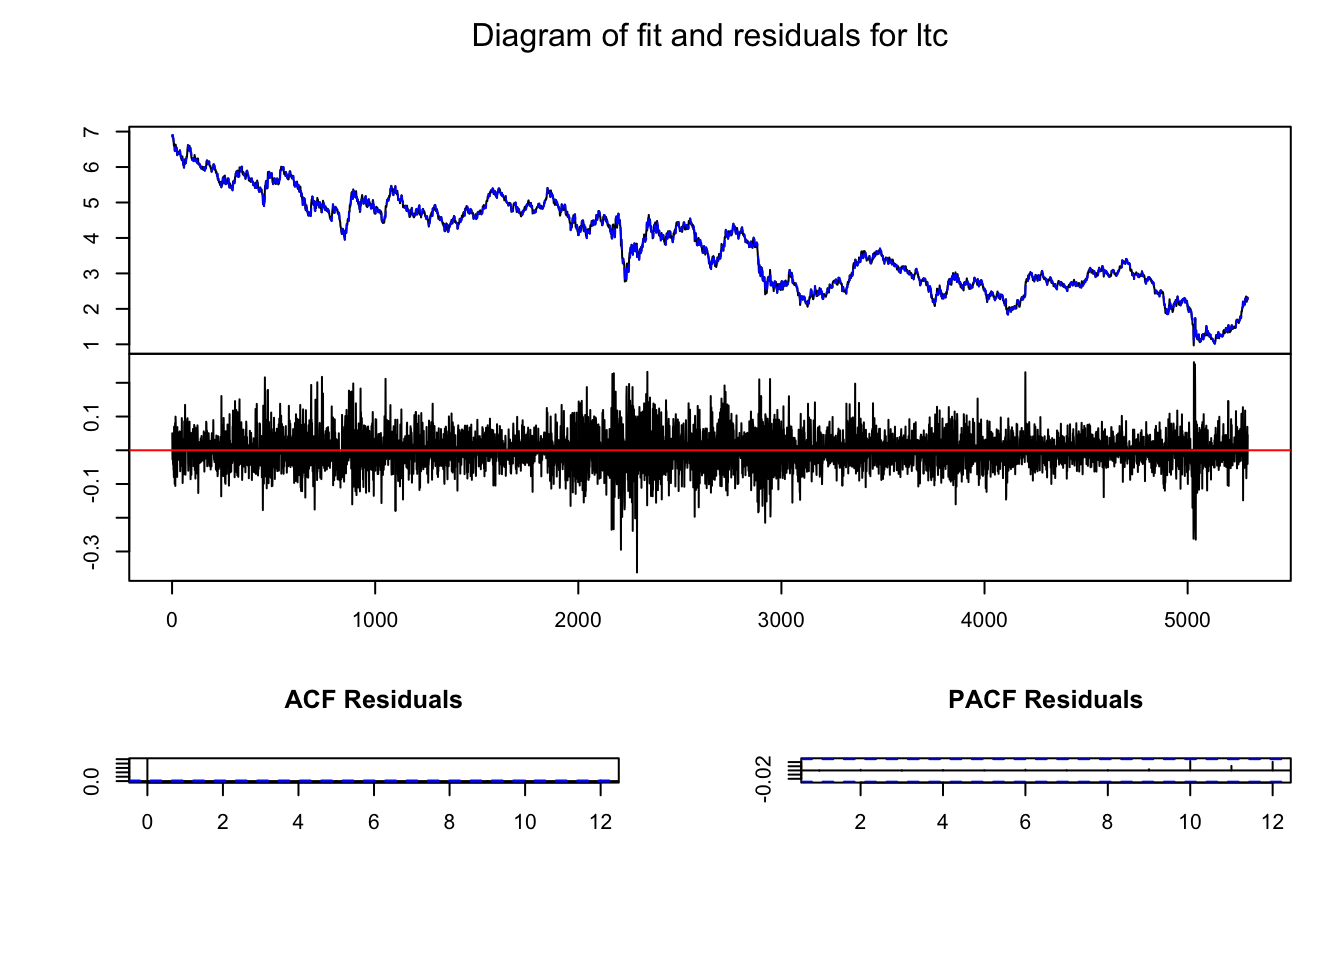
\includegraphics[width=0.8\textwidth]{../figuras-log/var-ltc.png}
\caption{\label{fig:residuales-var}Gráfica de los residuales, su autocorrelación y su autocorrelación parcial para las estimaciones del modelo VAR, para las ecuaciones de la variable \texttt{sp500} (arriba) y \texttt{ltc} (abajo).}
\end{figure}

Finalmente, en las figuras (\ref{fig:ir-sp500}) y (\ref{fig:ir-ltc}) se muestran las gráficas de impulso-respuesta para choques unitarios al sistema, tanto para la variable \texttt{sp500} como  para la variable \texttt{ltc} (consideradas como variables dependientes, respectivamente).

\begin{figure}[H]
\centering
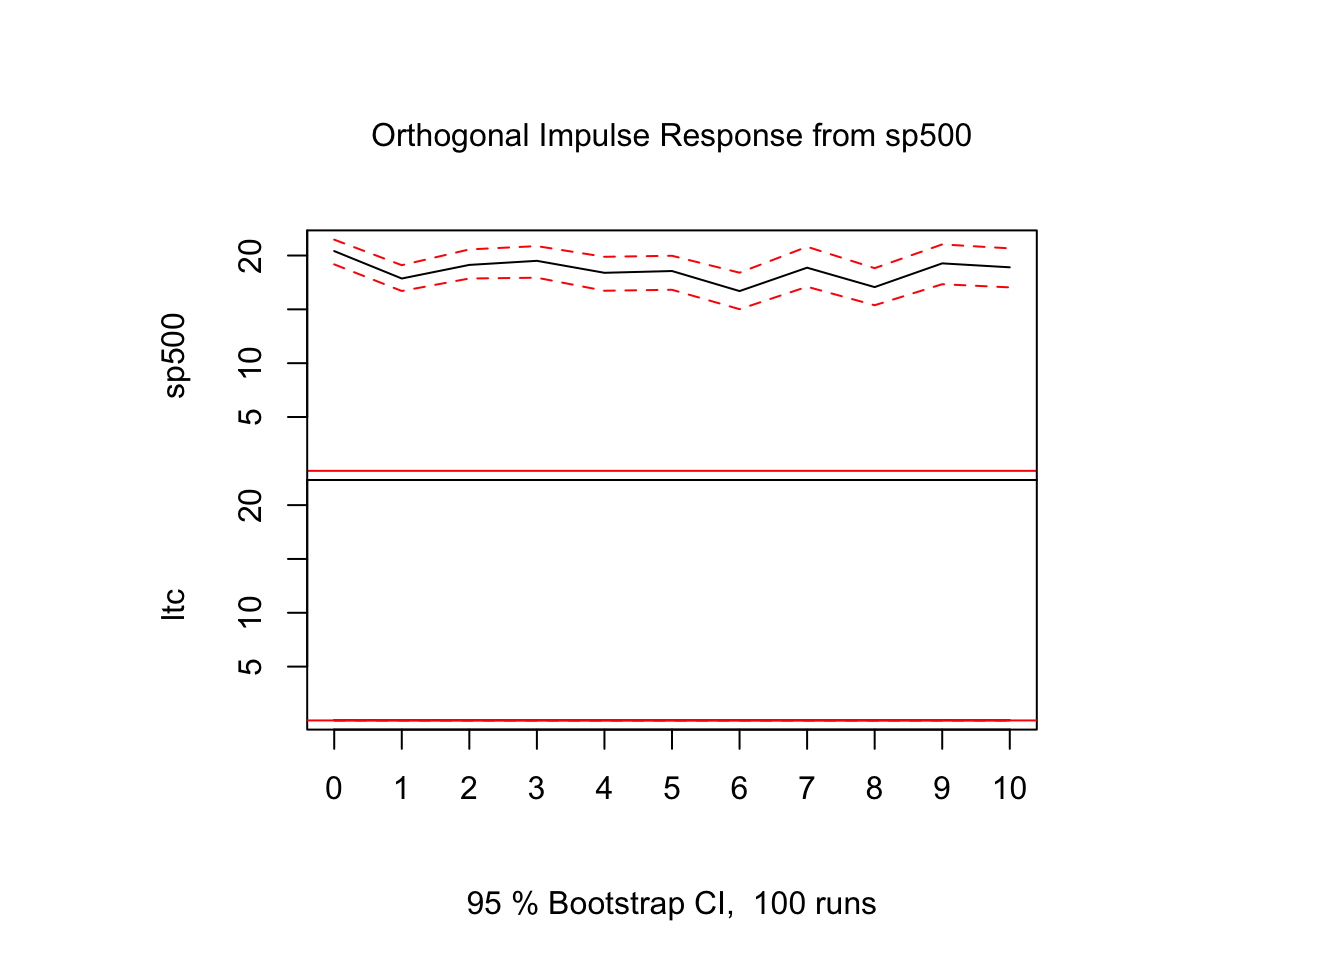
\includegraphics[width=0.8\textwidth]{../figuras-log/ir_sp500.png}
\caption{\label{fig:ir-sp500}Gráfica de impulso-respuesta para choques unitarios al sistema, como respuesta de la variable \texttt{sp500}.}
\end{figure}

Se observa que al inducir un choque unitario en el sistema, ambas variables responden y los efectos persisten incluso hasta diez periodos después del choque. Esto se puede verificar examinando los valores de los coeficientes del sistema al introducir el choque unitario. Estos coeficientes se muestran en el cuadro (\ref{tab:ir-sp500}) para la variable \texttt{sp500} y en el cuadro (\ref{tab:ir-ltc}) para la  variable \texttt{ltc}.

\begin{table}[H]
\centering
\begin{tabularx}{0.6\textwidth}{YYY}
\toprule
Rezagos & \texttt{sp500} & \texttt{ltc} \\
\midrule
1&20.41322&0.01736539\\
2&17.86466&0.01504078\\
3&19.1288&0.01469069\\
4&19.50848&0.01375604\\
5&18.39539&0.01204305\\
6&18.56075&0.01236441\\
7&16.69747&0.01310932\\
8&18.86988&0.01347808\\
9&17.06684&0.01249074\\
10&19.27205&0.01472273\\
11&18.90516&0.0142297\\
\bottomrule
\end{tabularx}
\caption{\label{tab:ir-sp500}Respuestas a un impulso unitario (variable dependiente: \texttt{sp500}).}
\end{table}

\begin{figure}[H]
\centering
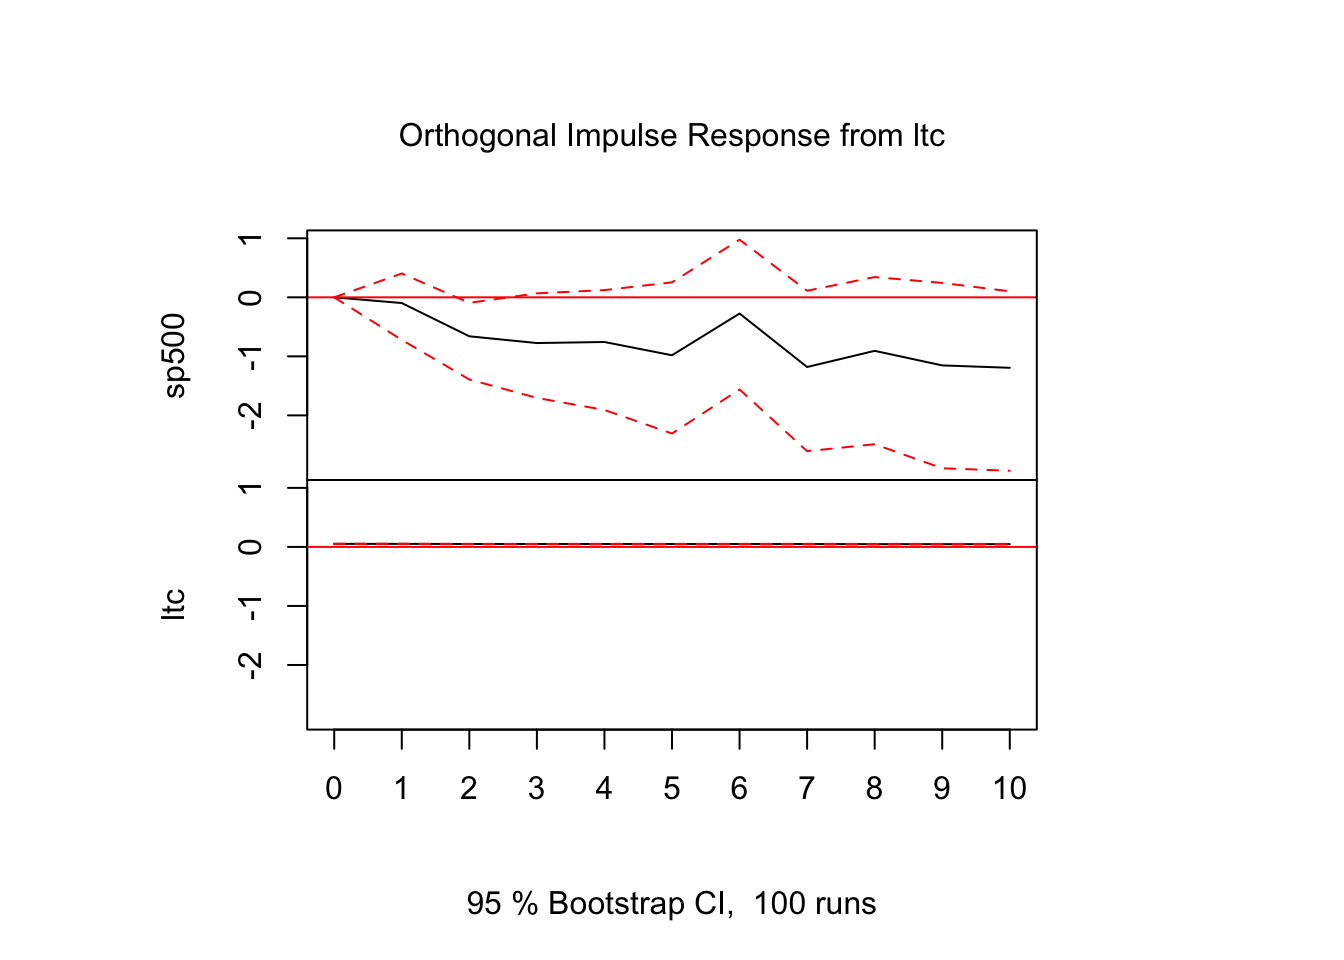
\includegraphics[width=0.8\textwidth]{../figuras-log/ir_ltc.png}
\caption{\label{fig:ir-ltc}Gráfica de impulso-respuesta para choques unitarios al sistema, como respuesta de la variable \texttt{ltc}.}
\end{figure}

\begin{table}[H]
\centering
\begin{tabularx}{0.6\textwidth}{YYY}
\toprule
Rezagos & \texttt{sp500} & \texttt{ltc} \\
\midrule
1&0&0.05162921\\
2&-0.09699875&0.05188628\\
3&-0.66037459&0.04932462\\
4&-0.77465724&0.04908652\\
5&-0.75664287&0.04898153\\
6&-0.98155554&0.04869442\\
7&-0.27452383&0.0487309\\
8&-1.18072949&0.04871283\\
9&-0.90665051&0.0469771\\
10&-1.15325776&0.04664313\\
11&-1.19386703&0.04671415\\
\bottomrule
\end{tabularx}
\caption{\label{tab:ir-ltc}Respuestas a un impulso unitario (variable dependiente: \texttt{ltc}).}
\end{table}

\end{document}
